\documentclass[12pt,letterpaper]{article}
\usepackage{geometry}
\geometry{letterpaper}
\usepackage{amsmath,amssymb,amsthm,mathrsfs}
\usepackage{mathtools}
\usepackage{ifpdf}
  \ifpdf
    \setlength{\pdfpagewidth}{8.5in}
    \setlength{\pdfpageheight}{11in}
  \else
\fi
\usepackage{hyperref}

\usepackage{tikz}
\usepackage{tikz-cd}
\usetikzlibrary{decorations.markings}
\tikzset{
  open/.style = {decoration = {markings, mark = at position 0.5 with { \node[transform shape] {\tikz\draw[fill=white] (0,0) circle (.3ex);}; } }, postaction = {decorate} },
  closed/.style = {decoration = {markings, mark = at position 0.5 with { \node[transform shape, xscale = .8, yscale=.4] {\upshape{/}}; } }, postaction = {decorate} },
  imm/.style = {decoration = {markings, mark = at position 0.3 with { \node[transform shape, xscale = .8, yscale=.4] {\upshape{/}}; }, mark = at position 0.6 with { \node[transform shape] {\tikz\draw[fill=white] (0,0) circle (.3ex);}; } }, postaction = {decorate} }
}

\usepackage{braket}

\usepackage[utf8]{inputenc}
\usepackage{csquotes}
\usepackage[american]{babel}
\usepackage[style=alphabetic,firstinits=true,backend=biber,texencoding=utf8,bibencoding=utf8]{biblatex}
\bibliography{../../References.bib}
\AtEveryBibitem{\clearfield{url}}
\AtEveryBibitem{\clearfield{doi}}
\AtEveryBibitem{\clearfield{issn}}
\AtEveryBibitem{\clearfield{isbn}}
\renewbibmacro{in:}{}
\DeclareFieldFormat{postnote}{#1}
\DeclareFieldFormat{multipostnote}{#1}

\renewcommand{\theenumi}{$(\alph{enumi})$}
\renewcommand{\labelenumi}{\theenumi}

\newcounter{enumacounter}
\newenvironment{enuma}
{\begin{list}{$(\alph{enumacounter})$}{\usecounter{enumacounter} \parsep=0em \itemsep=0em \leftmargin=2.75em \labelwidth=1.5em \topsep=0em}}
{\end{list}}
\newcounter{enumicounter}
\newenvironment{enumi}
{\begin{list}{$\roman{enumicounter})$}{\usecounter{enumicounter} \parsep=0em \itemsep=0em \leftmargin=2.25em \labelwidth=1.5em \topsep=0em}}
{\end{list}}
\newtheorem*{theorem}{Theorem}
\newtheorem*{universalproperty}{Universal Property}
\newtheorem{problem}{Exercise}[section]
\newtheorem{subproblem}{Problem}[problem]
\newtheorem{lemma}{Lemma}%[section]
\newtheorem{proposition}{Proposition}
\newtheorem{property}{Property}[problem]
\newtheorem*{lemma*}{Lemma}
\newtheorem*{claim}{Claim}
\theoremstyle{definition}
\newtheorem*{definition}{Definition}
\theoremstyle{remark}
\newtheorem*{remark}{Remark}

\numberwithin{figure}{problem}
\numberwithin{equation}{section}

\DeclareMathOperator{\Ann}{Ann}
\DeclareMathOperator{\Ass}{Ass}
\DeclareMathOperator{\Supp}{Supp}
\DeclareMathOperator{\WeakAss}{\widetilde{Ass}}
\let\Im\relax
\DeclareMathOperator{\Im}{im}
\DeclareMathOperator{\Spec}{Spec}
\DeclareMathOperator{\SPEC}{\mathbf{Spec}}
\DeclareMathOperator{\Sp}{sp}
\DeclareMathOperator{\Max}{Max}
\DeclareMathOperator{\maxSpec}{maxSpec}
\DeclareMathOperator{\Hom}{Hom}
\DeclareMathOperator{\Soc}{Soc}
\DeclareMathOperator{\Ht}{ht}
\DeclareMathOperator{\A}{\mathcal{A}}
\DeclareMathOperator{\V}{\mathbf{V}}
\DeclareMathOperator{\Aut}{Aut}
\DeclareMathOperator{\Char}{char}
\DeclareMathOperator{\Frac}{Frac}
\DeclareMathOperator{\Proj}{Proj}
\DeclareMathOperator{\stimes}{\text{\footnotesize\textcircled{s}}}
\DeclareMathOperator{\End}{End}
\DeclareMathOperator{\Ker}{Ker}
\DeclareMathOperator{\Coker}{coker}
\DeclareMathOperator{\LCM}{LCM}
\DeclareMathOperator{\Div}{Div}
\DeclareMathOperator{\id}{id}
\DeclareMathOperator{\Cl}{Cl}
\DeclareMathOperator{\dv}{div}
\DeclareMathOperator{\Gr}{Gr}
\DeclareMathOperator{\pr}{pr}
\DeclareMathOperator{\trd}{tr.d.}
\DeclareMathOperator{\rank}{rank}
\DeclareMathOperator{\codim}{codim}
\DeclareMathOperator{\sgn}{sgn}
\DeclareMathOperator{\GL}{GL}
\DeclareMathOperator{\lt}{lt}
\DeclareMathOperator{\lc}{lc}
\newcommand{\GR}{\mathbb{G}\mathrm{r}}
\newcommand{\gR}{\mathrm{Gr}}
\newcommand{\EE}{\mathscr{E}}
\newcommand{\FF}{\mathscr{F}}
\newcommand{\GG}{\mathscr{G}}
\newcommand{\HH}{\mathscr{H}}
\newcommand{\II}{\mathscr{I}}
\newcommand{\LL}{\mathscr{L}}
\newcommand{\MM}{\mathscr{M}}
\newcommand{\OO}{\mathcal{O}}
\newcommand{\Ss}{\mathscr{S}}
\newcommand{\Af}{\mathfrak{A}}
\newcommand{\Aa}{\mathscr{A}}
\newcommand{\PP}{\mathcal{P}}
\newcommand{\red}{\mathrm{red}}
\newcommand{\Sh}{\mathfrak{Sh}}
\newcommand{\Psh}{\mathfrak{Psh}}
\newcommand{\LRS}{\mathsf{LRS}}
\newcommand{\Sch}{\mathfrak{Sch}}
\newcommand{\Var}{\mathfrak{Var}}
\newcommand{\Rings}{\mathfrak{Rings}}
\DeclareMathOperator{\In}{in}
\DeclareMathOperator{\Ext}{Ext}
\DeclareMathOperator{\Spe}{Sp\acute{e}}
\DeclareMathOperator{\HHom}{\mathscr{H}\!\mathit{om}}
\newcommand{\isoto}{\overset{\sim}{\to}}
\newcommand{\isolongto}{\overset{\sim}{\longrightarrow}}
\newcommand{\Mod}{\mathsf{mod}\mathchar`-}
\newcommand{\MOD}{\mathsf{Mod}\mathchar`-}
\newcommand{\gr}{\mathsf{gr}\mathchar`-}
\newcommand{\qgr}{\mathsf{qgr}\mathchar`-}
\newcommand{\uqgr}{\underline{\mathsf{qgr}}\mathchar`-}
\newcommand{\qcoh}{\mathsf{qcoh}\mathchar`-}
\newcommand{\Alg}{\mathsf{Alg}\mathchar`-}
\newcommand{\coh}{\mathsf{coh}\mathchar`-}
\newcommand{\vect}{\mathsf{vect}\mathchar`-}
\newcommand{\imm}[1][imm]{\hspace{0.75ex}\raisebox{0.58ex}{%
\begin{tikzpicture}[commutative diagrams/every diagram]
\draw[commutative diagrams/.cd, every arrow, every label,hook,{#1}] (0,0ex) -- (2.25ex,0ex);
\end{tikzpicture}}\hspace{0.75ex}}
\newcommand{\dashto}[2]{\smash{\hspace{-0.7em}\begin{tikzcd}[column sep=small,ampersand replacement=\&] {#1} \rar[dashed] \& {#2} \end{tikzcd}\hspace{-0.7em}}}

%\usepackage{todonotes}
%\usepackage[notref,notcite]{showkeys}

\title{Atiyah-Macdonald Ch.~1 Rings and Ideals}
\author{Takumi Murayama and Kyu Jun}

\begin{document}
\maketitle
\setcounter{section}{1}
\begin{problem}\label{exc:1.1}
  Let $x$ be a nilpotent element of a ring $A$.
  Show that $1 + x$ is a unit of $A$.
  Deduce that the sum of a nilpotent element and a unit is a unit.
\end{problem}
\begin{proof}
  Suppose $x^n = 0$, and let $y = \sum_{i=0}^{n-1} (-x)^i$.
  Then, $(1+x)y = 1$.
  Now if $u \in A^\times$, we see $(u^{-1}x)^n = 0$.
  Thus, $u+x = u(1+u^{-1}x)$ is a unit since each factor is.
\end{proof}

\begin{problem}\label{exc:1.2}
  Let $A$ be a ring and let $A[x]$ be the ring of polynomials in an
  indeterminate $x$, with coefficients in $A$.
  Let $f = a_0 + a_1x + \cdots + a_nx^n \in A[x]$.
  Prove that
  \begin{enumi}
    \item $f$ is a unit in $A[x] \Leftrightarrow a_0$ is a unit in $A$
      and $a_1,\ldots,a_n$ are nilpotent.
    \item $f$ is nilpotent $\Leftrightarrow a_0,a_1,\ldots,a_n$ are nilpotent.
    \item $f$ is a zero-divisor $\Leftrightarrow$ there exists $a \ne 0$
      in $A$ such that $af = 0$.
    \item $f$ is said to be \emph{primitive} if $(a_0,a_1,\ldots,a_n) = (1)$.
      Prove that if $f,g \in A[x]$, then $fg$ is primitive
      $\Leftrightarrow f$ and $g$ are primitive.
  \end{enumi}
\end{problem}
\begin{proof}[Proof of $i)$]
  $\Rightarrow$. We induce on the degree $n$ of $f$.
  If $n=0$, then $f = a_0 \in A^\times$.
  So suppose $n > 0$.
  Let $b_0 + b_1x + \cdots + b_mx^m$ be the inverse of $f$.
  By matching degrees in $x$ in the equation $fg = 1$, we have the system of
  equations
  \begin{equation}\label{eq:1.2}
    \begin{aligned}
      a_nb_m &= 0\\
      a_{n-1}b_m + a_nb_{m-1} &= 0\\
      a_{n-2}b_m + a_{n-1}b_{m-1} + a_nb_{m-2} &= 0\\
      &\ \,\vdots\\
      a_0b_0 &= 1.
    \end{aligned}
  \end{equation}
  The last row gives that $a_0,b_0$ are units.
  We now claim that $a_n^{r+1}b_{m-r} = 0$ for $0 \le r \le m$.
  The case when $r=0$ is the first row in \eqref{eq:1.2}.
  Suppose the claim holds for all $0 \le r < k$.
  We then have
  \begin{multline*}
    a_n^k(a_{n-k}b_m + a_{n-k+1}b_{m-1} + \cdots + a_{n-1}b_{m-k+1} + a_nb_{m-k})\\
    = a_n^ka_{n-k}b_m + a_n^ka_{n-k+1}b_{m-1} + \cdots + a_n^ka_{n-1}b_{m-k+1} + a_n^{k+1}b_{m-k} = 0
  \end{multline*}
  by multiplying the $(k+1)$th line from \eqref{eq:1.2} by $a_n^k$.
  All but the last term vanish by inductive hypothesis, and so
  $a_n^{k+1}b_{m-k} = 0$.
  In particular, for $r=m$ we have $a_n^{m+1}b_0 = 0$, which implies
  $a_n^{m+1} = 0$ since $b_0$ is a unit, i.e., $a_n$ is nilpotent. 
  Now $f - a_nx^n$ is a unit by Exercise \ref{exc:1.1}, hence by inductive
  hypothesis $a_1,\ldots,a_{n-1}$ are units as well.
  \par $\Leftarrow$. $g = \sum_{i=1}^n a_ix^i$ is nilpotent since $\mathfrak{N}$
  is an ideal by Prop.~1.7, so $f = a_0 + g$ is a unit by Exercise \ref{exc:1.1}.
\end{proof}
\begin{proof}[Proof of $ii)$]
  $\Rightarrow$. $1 + f$ is a unit by Exercise \ref{exc:1.1}, and so
  $a_1,\ldots,a_n$ are nilpotent by $i)$.
  $a_0$ is nilpotent as well for otherwise $f^m$ has constant term $a_0^m \ne 0$
  for any $m$.
  \par $\Leftarrow$. If $a_0,a_1,\ldots,a_n \in \mathfrak{N}$, $f \in \mathfrak{N}$
  since $\mathfrak{N}$ is an ideal by Prop.~1.7.
\end{proof}
\begin{proof}[Proof of $iii)$]
  $\Leftarrow$. Trivial since $a \in A \subset A[x]$.
  \par $\Rightarrow$. Suppose not, and let $g = b_0 + b_1x + \cdots + b_mx^m$
  be a polynomial of least degree $m > 0$ such that $fg = 0$.
  We claim $a_{n-r}g = 0$ for all $0 \le r \le n$.
  First, $a_nb_m=0$, hence $a_ng = 0$ since it has degree less than $m$ but
  annihilates $f$. Now suppose that $a_{n-r}g = 0$ for all $0 \le r < r_0$.
  Then, we have that
  \begin{equation*}
    fg = \left(a_0 + a_1x + \cdots + a_{n-r_0}x^{n-r_0}\right)g = 0
  \end{equation*}
  by inductive hypothesis.
  Then, $a_{n-r_0}b_m = 0$, hence $a_{n-r_0}g = 0$ since it has degree less than $m$ 
  but annihilates $f$.
  By induction, $a_{n-r}g = 0$ for all $0 \le r \le n$, hence letting $a = b_m$
  gives $af = 0$, a contradiction.
\end{proof}
\begin{proof}[Proof of $iv)$]
  $\Rightarrow$. Suppose $fg$ is primitive but $f$ is not.
  Then, $\mathfrak{a} = (a_0,a_1,\ldots,a_n) \subset \mathfrak{m} \subsetneq A$
  by Cor.~$1.4$, where $\mathfrak{m}$ is a maximal ideal.
  Now consider the natural homomorphism $\varphi\colon A[x] \to A/\mathfrak{m}[x]$
  induced by the map $A \to A/\mathfrak{m}$ on coefficients.
  $\varphi(f) = 0$ implies that $\varphi(fg) = 0$, and so the coefficients of $fg$
  are in $\mathfrak{m}$, a contradiction.
  \par $\Leftarrow$. Suppose $f,g$ are primitive but $fg$ is not.
  Then, the coefficients of $fg$ generate an ideal $\mathfrak{a}$, and
  $\mathfrak{a} \subset \mathfrak{m} \subsetneq A$ by Cor.~$1.4$, where
  $\mathfrak{m}$ is again a maximal ideal.
  The same map $\varphi$ defined above has $\varphi(fg) = 0$, and so
  $\varphi(f)\varphi(g) = 0$, i.e., either $\varphi(f) = 0$ or $\varphi(g) = 0$,
  for if either were a zero divisor, then there exists $a \in A/\mathfrak{m}$ such
  that $a\varphi(f) = 0$ by $iii)$, contradicting that $A/\mathfrak{m}$ is a field.
  Thus, the coefficients of either $f$ or $g$ are contained in $\mathfrak{m}$,
  a contradiction. 
\end{proof}

\begin{problem}
  Generalize the results of Exercise $\hyperref[exc:1.2]{2}$ to a polynomial ring
  $A[x_1,\ldots,x_r]$ in several indeterminates.
\end{problem}
\begin{claim}
  Let $A$ be a ring and let $A[x_1,\ldots,x_r]$ be the ring of polynomials in
  several indeterminates $x_1,\ldots,x_r$, with coefficients in $A$.
  Let $f \in A[x_1,\ldots,x_r]$. Then,
  \begin{enumi}
    \item $f$ is a unit in $A[x_1,\ldots,x_r] \Leftrightarrow$ its constant term
      $a_0$ is a unit in $A$ and all other coefficients are nilpotent.
    \item $f$ is nilpotent $\Leftrightarrow$ all its coefficients are nilpotent.
    \item $f$ is a zero-divisor $\Leftrightarrow$ there exists $a \ne 0$ in $A$
      such that $af = 0$.
    \item If $f,g \in A[x_1,\ldots,x_r]$, then $fg$ is primitive
      $\Leftrightarrow f$ and $g$ are primitive.
  \end{enumi}
\end{claim}
\begin{proof}[Proof of $i),ii)$]
  We induce on $r$. $r=1$ is Exercise \ref{exc:1.2}.
  Now consider$A[x_1,\ldots,x_r]$ as a polynomial ring in an indeterminate $x_r$
  over the ring $A[x_1,\ldots,x_{r-1}]$, and write $f = \sum f_ix_r^i$, where
  $f_i \in A[x_1,\ldots,x_{r-1}]$.
  By Exercise \ref{exc:1.2}, $f$ is a unit (resp.~nilpotent) if and only if $f_0$
  is a unit and $f_1,\ldots,f_n$ are nilpotent (resp.~each coefficient $f_i$ is
  nilpotent).
  By inductive hypothesis, this is equivalent to the constant term $a_0$ of $f_0$
  being a unit and each other coefficient of $f_i$ in $A$ being nilpotent
  (resp.~every coefficient of the $f_i$ in $A$ being nilpotent).
\end{proof}
\begin{proof}[Proof of $iii)$]
  $\Rightarrow$. Trivial since $a \in A \subset A[x_1,\ldots,x_r]$.
  \par $\Leftarrow$. Suppose not.
  Using multi-index notation $x^\alpha = x_1^{\alpha^1}\cdots x_r^{\alpha^r}$
  where $\alpha = (\alpha^1,\ldots,\alpha^r) \in \mathbb{N}^r$, consider the
  well-ordering $\succ$ on monomials in $A[x_1,\ldots,x_r]$ defined by
  $\alpha \succ \beta$ if the left-most nonzero entry in $\alpha - \beta$ is
  positive (the \emph{lexicographic} order).
  Define $\lt(f)$ to be the leading term of $f$ with respect to $\succ$, and
  $\lc(f)$ to be the coefficient of $\lt(f)$.
  Now write $f = a_{n}x^{\alpha_n} + a_{n-1}x^{\alpha_{n-1}} +
  \cdots + a_{0}x^{\alpha_0}$ where $\alpha_n \succ \alpha_{n-1} \succ
  \cdots \succ \alpha_0$.
  Let $g$ be a polynomial $fg = 0$ such that $\lt(g)$ is minimal with respect to
  $\succ$.
  We claim $a_{n-s}g = 0$ for all $0 \le s \le n$.
  First, $\lc(fg) = \lc(f)\lc(g) = 0$, hence $a_ng = 0$ since $g \succ a_ng$
  but $f \cdot a_{n-s_0}g = 0$.
  Now suppose that $a_{n-s}g = 0$ for all $0 \le s < s_0$. Then, we have that
  \begin{equation*}
    fg = \left( a_{n-s_0}x^{\alpha_{n-s_0}} + \cdots + a_0x^{\alpha_{0}} \right)g = 0
  \end{equation*}
  by inductive hypothesis.
  Then, $a_{n-s_0}\lc(g) = 0$, hence $a_{n-s_0}g = 0$ since $g \succ a_{n-s_0}g$
  but $f \cdot a_{n-s_0}g = 0$.
  By induction, $a_{n-s}g = 0$ for all $0 \le s \le n$, hence letting
  $a = \lc(g)$ gives $af = 0$, a contradiction.
\end{proof}
\begin{proof}[Proof of $iv)$]
  $\Rightarrow$. Suppose $fg$ is primitive but $f$ is not.
  Then, the coefficients of $f$ generate an ideal
  $\mathfrak{a} \subset \mathfrak{m} \subsetneq A$ by Cor.~$1.4$, where
  $\mathfrak{m}$ is a maximal ideal.
  Now consider the natural homomorphism
  $\varphi\colon A[x_1,\ldots,x_r] \to A/\mathfrak{m}[x_1,\ldots,x_r]$
  induced by the map $A \to A/\mathfrak{m}$ on coefficients.
  $\varphi(f) = 0$ implies that $\varphi(fg) = 0$, and so the coefficients of
  $fg$ are in $\mathfrak{m}$, a contradiction.
  \par $\Leftarrow$. Suppose $f,g$ are primitive but $fg$ is not.
  Then, the coefficients of $fg$ generate an ideal $\mathfrak{a}$, and
  $\mathfrak{a} \subset \mathfrak{m} \subsetneq A$ by Cor.~$1.4$, where
  $\mathfrak{m}$ is again a maximal ideal.
  The same map $\varphi$ defined above has $\varphi(fg) = 0$, and so
  $\varphi(f)\varphi(g) = 0$, i.e., either $\varphi(f) = 0$ or $\varphi(g) = 0$,
  for if either were a zero divisor, then there exists $a \in A/\mathfrak{m}$
  such that $a\varphi(f) = 0$ by $iii)$, contradicting that $A/\mathfrak{m}$ is
  a field.
  Thus, the coefficients of either $f$ or $g$ are contained in $\mathfrak{m}$, a contradiction. 
\end{proof}

\begin{problem}\label{exc:1.4}
  In the ring $A[x]$, the Jacobson radical is equal to the nilradical.
\end{problem}
\begin{proof}
  Since every maximal ideal is prime, Prop.~1.8 implies $\mathfrak{N} \subset \mathfrak{R}$. Conversely, suppose $f = a_0 + a_1x + \cdots + a_nx^n \in \mathfrak{R}$. By Prop.~1.9, $1-fx$ is a unit. By Exercise $\ref{exc:1.2}i)$, the $a_i$ are nilpotent, and so $f \in \mathfrak{N}$ by Exercise $\ref{exc:1.2}ii)$.
\end{proof}

\begin{problem}
  Let $A$ be a ring and let $A[[x]]$ be the ring of formal power series $f = \sum_{n=0}^\infty a_nx^n$ with coefficients in $A$. Show that
  \begin{enumi}
    \item $f$ is a unit in $A[[x]] \Leftrightarrow a_0$ is a unit in $A$.
    \item If $f$ is nilpotent, then $a_n$ is nilpotent for all $n \ge 0$. Is the converse true? (See \href{AM 7 Noetherian Rings.pdf#exc:7.2}{Chapter $7$, Exercise $2$}.)
    \item $f$ belongs to the Jacobson radical of $A[[x]] \Leftrightarrow a_0$ belongs to the Jacobson radical of $A$.
    \item The contraction of a maximal ideal $\mathfrak{m}$ of $A[[x]]$ is a maximal ideal of $A$, and $\mathfrak{m}$ is generated by $\mathfrak{m}^c$ and $x$.
    \item Every prime ideal of $A$ is the contraction of a prime ideal of $A[[x]]$.
  \end{enumi}
\end{problem}
\begin{proof}[Proof of $i)$]
  Write $g = \sum_{n=0}^\infty b_nx^n$.
  \par $\Rightarrow$. Any unit $f$ must have $a_0 \in A^\times$, for $fg = 1$ implies $a_0b_0 = 1$.
  \par $\Leftarrow$. Define $g$ recursively where $b_0 = a_0^{-1}$, and 
    $b_i = -a_0^{-1}\sum_{j=1}^i a_jb_{i-j}$ for $i>0$.
  Then, $a_0b_0 = 1$, and $fg = 1$ since all other coefficients are of the form
  \begin{equation*}
    \sum_{i=0}^k a_{k-i}b_{i} = a_0b_k + a_1b_{k-1} + a_2b_{k-2} + \cdots + a_kb_0 = 0.\qedhere
  \end{equation*}
\end{proof}
\begin{proof}[Proof of $ii)$]
  Suppose $f \in \mathfrak{N}$; we claim $a_n \in \mathfrak{N}$ by induction on $n$. $f^N = 0$ implies $a_0^N = 0$ by looking at the coefficient of least degree. Now suppose $a_n \in \mathfrak{N}$ for all $n < n_0$. Then, $f - a_0 - a_1x - \cdots - a_{n_0-1}x^{n_0} \in \mathfrak{N}$ by inductive hypothesis since $\mathfrak{N}$ is an ideal by Prop.~1.7. If $(f - a_0 - a_1x - \cdots - a_{n_0-1}x^{n_0})^N = 0$, then $a_{n_0}^N = 0$ by looking at the coefficient of least degree, hence by induction $a_n$ is nilpotent for $n \ge 0$.
  \par We claim the converse is false. Let $A = \prod_{i=0}^\infty \mathbb{Z}/(2^{i+2})$ and $a_n \in A$ such that $p_i(a_n) = 2\delta_{in}$, where $p_i$ are the projection maps $A \to \mathbb{Z}/(2^{i+2})$. Then, $a_n \in \mathfrak{N}$ for $n \ge 0$, and since $a_na_m = 0$ if $n \ne m$, letting $f = \sum_{n=0}^\infty a_nx^n$, we see for any $N$,
  \begin{equation*}
    f^N = a_0^N + a_1^Nx^N + a_2^Nx^{2N} + \cdots \ne 0.\qedhere
  \end{equation*}
\end{proof}
\begin{proof}[Proof of $iii)$]
  $f \in \mathfrak{R}_{A[[x]]}$ if and only if $1 - fg \in A[[x]]^\times$ for all $g \in A[[x]]$ by Prop.~1.9. By $i)$, this holds if and only if $1-a_0b_0 \in A^\times$ for $b_0 \in A$ by considering $g = b_0 + xg'$. This is true if and only if $a_0 \in \mathfrak{R}_A$ by Prop.~1.9.
\end{proof}
\begin{proof}[Proof of $iv)$]
  It suffices to show $A/\mathfrak{m}^c$ is a field. By $iii)$, $x \in \mathfrak{R}_{A[[x]]} \subseteq \mathfrak{m}$ for any maximal ideal $\mathfrak{m} \subseteq A[[x]]$ since $0 \in \mathfrak{R}_A$. Now if $0 \ne a \in A$, then since $A[[x]]/\mathfrak{m}$ is a field, there exists $a_0 + xg \in A[[x]]$ such that $a(a_0 + xg) \equiv 1 \bmod \mathfrak{m}$. Since $x \in \mathfrak{m}$, $aa_0 \equiv a(a_0 + xg) \bmod \mathfrak{m}$, hence $aa_0 \equiv 1 \bmod \mathfrak{m}^c$.
  \par Now $(\mathfrak{m}^c,x) \subseteq \mathfrak{m}$ since $a_0 \in \mathfrak{m}^c$ and $x \in \mathfrak{m}$ imply $a_0f + gx \in \mathfrak{m}$. Conversely, if $f = a_0 + gx \in \mathfrak{m}$, then $a_0 = f - gx \in \mathfrak{m}^c$ since $x \in \mathfrak{m}$, hence $\mathfrak{m} \subseteq (\mathfrak{m}^c,x)$.
\end{proof}
\begin{proof}[Proof of $v)$]
  Suppose $\mathfrak{p} \subseteq A$ is a prime ideal; then, the ideal $\mathfrak{q} \coloneqq (\mathfrak{p},x)$ of $f \in A[[x]]$ with $a_0 \in \mathfrak{p}$ is prime since $fg \in \mathfrak{q}$ implies $a_0b_0 \in \mathfrak{p}$, and so either $f$ or $g$ is in $\mathfrak{q}$. Since $\mathfrak{p} = \mathfrak{q}^c$, we are done.
\end{proof}

\begin{problem}
  A ring $A$ is such that every ideal not contained in the nilradical contains a non-zero idempotent (that is, an element $e$ such that $e^2 = e \ne 0$). Prove that the nilradical and Jacobson radical of $A$ are equal.
\end{problem}
\begin{proof}
  $\mathfrak{N} \subseteq \mathfrak{R}$ as in Exercise \ref{exc:1.4}. Conversely, suppose there exists a non-zero idempotent $e \in \mathfrak{R} \setminus \mathfrak{N}$. Then, $e(1-e) = e - e^2 = e-e = 0$. By Prop.~$1.9$, $1-e$ is a unit. But then, $0 = 0(1-e)^{-1} = e(1-e)(1-e)^{-1} = e$, which is a contradiction.
\end{proof}

\begin{problem}\label{exc:1.7}
  Let $A$ be a ring in which every element $x$ satisfies $x^n = x$ for some $n > 1$ (depending on $x$). Show that every prime ideal in $A$ is maximal.
\end{problem}
\begin{proof}
  Let $\mathfrak{p} \subseteq A$ be a prime ideal, and consider $x \in A \setminus \mathfrak{p}$. Let $\overline{x}$ be the residue of $x$ in $A/\mathfrak{p}$. Then, $\overline{x}^n = \overline{x}$, so $\overline{x}(1-\overline{x}^{n-1}) = \overline{x} - \overline{x}^n = 0$. Since $\mathfrak{p}$ prime implies $A/\mathfrak{p}$ is a domain and $\overline{x} \ne 0$ by choice of $x$, we then have $\overline{x}^{n-1} = 1$. Thus, $\overline{x}\overline{x}^{n-2} = 1$, and so every $0 \ne \overline{x} \in A/\mathfrak{p}$ is a unit, i.e., $A/\mathfrak{p}$ is a field. Thus, $\mathfrak{p}$ is maximal.
\end{proof}

\begin{problem}\label{exc:1.8}
  Let $A$ be a ring $\ne 0$. Show that the set of prime ideals of $A$ has minimal elements with respect to inclusion.
\end{problem}
\begin{proof}
  We order the set $\Spec A$ of prime ideals by reverse inclusion. $\Spec A \ne \emptyset$ by Thm.~$1.3$. By Zorn's lemma, it suffices to show for every descending chain of prime ideals $\{\mathfrak{p}_\alpha\}$ in $\Spec A$, the lower bound $\mathfrak{p} = \bigcap_\alpha \mathfrak{p}_\alpha$ is in $\Spec A$. If $xy \in \mathfrak{p}$, then $xy \in \mathfrak{p}_\alpha$ for all $\alpha$, and so for any $\alpha$, either $x \in \mathfrak{p}_\alpha$ or $y \in \mathfrak{p}_\alpha$. Since $\mathfrak{p}_\alpha$ are a descending chain, at least one of $x,y$ is in the intersection $\mathfrak{p}$. Thus, $\mathfrak{p} \in \Spec A$.
\end{proof}

\begin{problem}
  Let $\mathfrak{a}$ be an ideal $\ne (1)$ in a ring $A$. Show that $\mathfrak{a} = r(\mathfrak{a}) \Leftrightarrow \mathfrak{a}$ is an intersection of prime ideals.
\end{problem}
\begin{proof}
  $\Rightarrow$ follows by Prop.~1.14.
  \par $\Leftarrow$. Suppose $\mathfrak{a} = \bigcap \mathfrak{p}_i$. $\mathfrak{a} \subseteq r(\mathfrak{a})$ is true by definition. Since $\{\mathfrak{p}_i\} \subseteq \{\mathfrak{q}_k \mid \mathfrak{q}_k \supseteq \mathfrak{a}\}$ and by Prop.~$1.14$ $r(\mathfrak{a}) = \bigcap \mathfrak{q}_k$, we have $\mathfrak{a} \supseteq r(\mathfrak{a})$. Thus, $\mathfrak{a} = r(\mathfrak{a})$.
\end{proof}

\begin{problem}
  Let $A$ be a ring, $\mathfrak{N}$ its nilradical. Show that the following are equivalent:
  \begin{enumi}
    \item $A$ has exactly one prime ideal;
    \item every element of $A$ is either a unit or nilpotent;
    \item $A/\mathfrak{N}$ is a field.
  \end{enumi}
\end{problem}
\begin{proof}
  $i) \Rightarrow ii)$. $\mathfrak{p} = \mathfrak{N}$ by Prop.~1.8, so $x^n = 0$ for all $x \in \mathfrak{p}$. Now if $y \notin \mathfrak{p}$, it is a unit by the contrapositive of Cor.~1.5.
  \par $ii) \Rightarrow iii)$. If $x \in A/\mathfrak{N}$, it can be lifted to $\tilde{x} \in A \setminus \mathfrak{N}$, and so $x\overline{\tilde{x}^{-1}} = \overline{\tilde{x}\tilde{x}^{-1}} = 1$.
  \par $iii) \Rightarrow i)$. $\mathfrak{N}$ is a maximal ideal since $A/\mathfrak{N}$ is a field. By Prop.~8, $\mathfrak{N} \subseteq \mathfrak{p}$ for any prime ideal $\mathfrak{p} \subseteq A$. By maximality, $\mathfrak{N} = \mathfrak{p}$, so $\mathfrak{N}$ is the unique prime ideal in $A$.
\end{proof}

\begin{problem}\label{exc:1.11}
  A ring $A$ is \emph{Boolean} if $x^2 = x$ for all $x \in A$. In a Boolean ring $A$, show that
  \begin{enumi}
    \item $2x = 0$ for all $x \in A$;
    \item every prime ideal $\mathfrak{p}$ is maximal, and $A/\mathfrak{p}$ is a field with two elements;
    \item every finitely generated ideal in $A$ is principal.
  \end{enumi}
\end{problem}
\begin{proof}[Proof of $i)$]
  $x+x = (x+x)^2 = x^2 + 2x + x^2 = x+x+2x$, so $2x = 0$.
\end{proof}
\begin{proof}[Proof of $ii)$]
  Every prime ideal $\mathfrak{p}$ is maximal by Exercise \ref{exc:1.7}, so $A/\mathfrak{p}$ is a field. Now consider $x \in A \setminus \mathfrak{p}$, and let $\overline{x}$ be the residue of $x$ in $A/\mathfrak{p}$. Then, $x^2 = x$ implies $\overline{x}(\overline{x}-1) = 0$. But $A/\mathfrak{p}$ is a field, hence $\overline{x} = 0$ or $1$, i.e., $A/\mathfrak{p} = \{0,1\}$.
\end{proof}
\begin{proof}[Proof of $iii)$]
  We induce on the number of generators $n$ of an ideal $\mathfrak{a} \subseteq A$. Suppose $n=2$, and $\mathfrak{a} = (x,y)$. Then clearly $(x+y-xy) \subseteq \mathfrak{a}$, and $\mathfrak{a} \subseteq (x+y-xy)$ since $x(x+y-xy) = x^2+xy-x^2y = x$ and similarly $y(x+y-xy) = xy+y^2-xy^2 = y$. If $n>2$, let $\mathfrak{a} = (x,\mathfrak{a}')$; by inductive hypothesis, $\mathfrak{a}' = (y)$ for some $y$, and so $\mathfrak{a} = (x,y) = (x+y-xy)$ by the above.
\end{proof}

\begin{problem}\label{exc:1.12}
  A local ring contains no idempotent $\ne 0,1$.
\end{problem}
\begin{proof}
  Let $A$ be our local ring; by Cor.~$1.5$, $\mathfrak{R} = A \setminus A^\times$. If $e$ is idempotent, one of $e,1-e$ is a unit for otherwise $1 = e + (1-e) \in \mathfrak{R}$, a contradiction. Since $e$ is idempotent, $e(1-e) = 0$. So, if $e$ is a unit, then $0 = 0e^{-1} = (1-e)ee^{-1} = 1-e$ and $e = 1$; if $1-e$ is a unit, then $0 = 0(1-e)^{-1} = e(1-e)(1-e)^{-1} = e$ and $1-e = 1$.
\end{proof}

\begin{problem}
  Let $K$ be a field and let $\Sigma$ be the set of all irreducible monic polynomials $f$ in one indeterminate with coefficients in $K$. Let $A$ be the polynomial ring over $K$ generated by indeterminates $x_f$, one for each $f \in \Sigma$. Let $\mathfrak{a}$ be the ideal of $A$ generated by the polynomials $f(x_f)$ for all $f \in \Sigma$. Show that $\mathfrak{a} \ne (1)$.
  \par Let $\mathfrak{m}$ be a maximal ideal of $A$ containing $\mathfrak{a}$, and let $K_1 = A/\mathfrak{m}$. Then $K_1$ is an extension field of $K$ in which each $f \in \Sigma$ has a root. Repeat the construction with $K_1$ in place of $K$, obtaining a field $K_2$, and so on. Let $L = \bigcup_{n=1}^\infty K_n$. Then $L$ is a field in which each $f \in \Sigma$ splits completely into linear factors. Let $\overline{K}$ be the set of all elements of $L$ which are algebraic over $K$. Then $\overline{K}$ is an algebraic closure of $K$.
\end{problem}
\begin{proof}
  Suppose $\mathfrak{a} = (1)$, and so there exist $g_i \in A$ such that $\sum g_if_i(x_{f_i}) = 1$. The residue of this sum in $A/(f_1(x_{f_1}),\ldots,f_n(x_{f_n}))$ equals zero, which is a contradiction since $A/(f_1(x_{f_1}),\ldots,f_n(x_{f_n}))$ is isomorphic to the polynomial ring over the field $K[x_{f_1},\ldots,x_{f_n}]/(f_1(x_{f_1}),\ldots,f_n(x_{f_n}))$ with indeterminates $\{x_f \mid f \in \Sigma \setminus \{f_1,\ldots,f_n\}\}$.
  \par Every $f$ has a root $\alpha_1 \coloneqq x_f + \mathfrak{m} \in K_1$ since $f(\alpha_1) = f(x_f) + \mathfrak{m} = \mathfrak{m}$ in $A/\mathfrak{m}$.
  \par We claim if $f \in K[x]$ is of degree $m>0$, then it splits completely in $K_{m-1}$. We proceed by induction on $m$. This is clear if $m=1$ where $K_0 \coloneqq K$. If $m > 1$, by the above $f$ has a root $\alpha_1 \in K_{1}$, hence $f/(x-\alpha_1)$ has degree $m-1$ in $K_{1}$. By inductive hypothesis, $f/(x-\alpha_1)$ splits completely in $K_{m-1}$, hence $f$ splits completely in $K_{m-1}$.
  \par Now let $\overline{K}$ be the set of all elements in $L$ which are algebraic over $K$. It is a ring by Cor.~5.3, and moreover a field since if $\alpha$ is a root of $f$, then $\alpha^{-1}$ is a root of $x^{\deg f}f(x^{-1})$. It is algebraically closed since every polynomial $g \in K[x]$ has an irreducible factor $f$ which has a root in $\overline{K}$ by construction.
\end{proof}

\begin{problem}
  In a ring $A$, let $\Sigma$ be the set of all ideals in which every element is a zero-divisor. Show that the set $\Sigma$ has maximal elements and that every maximal element of $\Sigma$ is a prime ideal. Hence the set of zero-divisors in $A$ is a union of prime ideals.
\end{problem}
\begin{proof}
  We order $\Sigma$ by inclusion; $\Sigma \ne \emptyset$ since $(0) \in \Sigma$. By Zorn's lemma, to show $\Sigma$ has maximal elements it suffices to show for every ascending chain $\{\mathfrak{a}_\alpha\}$ in $\Sigma$, the upper bound $\mathfrak{a} = \bigcup_\alpha \mathfrak{a}_\alpha$ is in $\Sigma$. $\mathfrak{a}$ is an ideal since if $x,y \in \mathfrak{a}$, they are both in some $\mathfrak{a}_\alpha$, and so $x+y \in \mathfrak{a}_\alpha \subseteq \mathfrak{a}$; similarly, if $x \in \mathfrak{a}$, it is in some $\mathfrak{a}_\alpha$, and so $ax \in \mathfrak{a}_\alpha \subseteq \mathfrak{a}$ for any $a \in A$. Moreover, $\mathfrak{a} \in \Sigma$ since every element $x \in \mathfrak{a}$ must be contained in some $\mathfrak{a}_\alpha$ and so is a zero-divisor.
  \par We now show these maximal $\mathfrak{a} \in \Sigma$ are prime. So, suppose $xy \in \mathfrak{a}$ but $x,y \notin \mathfrak{a}$. Then, $\mathfrak{a} \subsetneq (\mathfrak{a} : x)$ since $y \notin \mathfrak{a}$. By maximality, $(\mathfrak{a} : x)$ contains some $z$ which is not a zero-divisor. We now claim that $(\mathfrak{a} : z) \in \Sigma$. If $0 \ne w \in (\mathfrak{a} : z)$, then $wz \in \mathfrak{a}$, hence there exists $v \in A$ such that $vwz = 0$. Since $z$ is not a zero-divisor, $vz \ne 0$, hence $w$ is a zero-divisor. But $\mathfrak{a} \subsetneq (\mathfrak{a} : z)$ since $x \in (\mathfrak{a} : z)$, contradicting the maximality of $\mathfrak{a}$.
  \par Now we show that the set of zero-divisors in $A$ is a union of prime ideals. If $x \in A$ is a zero-divisor, then $(x) \in \Sigma$. By repeating the argument in the first paragraph to the subset of $\Sigma$ of ideals containing $(x)$, we see that there is a maximal $\mathfrak{a} \in \Sigma$ such that $x \in \mathfrak{a}$. Thus, the set of zero-divisors in $A$ is the union of maximal elements in $\Sigma$, which are prime ideals.
\end{proof}

\begin{problem}\label{exc:1.15}
  Let $A$ be a ring and let $X$ be the set of all prime ideals of $A$. For each subset $E$ of $A$, let $V(E)$ denote the set of all prime ideals of $A$ which contain $E$. Prove that
  \begin{enumi}
    \item if $\mathfrak{a}$ is the ideal generated by $E$, then $V(E) = V(\mathfrak{a}) = V(r(\mathfrak{a}))$.
    \item $V(0) = X$, $V(1) = \emptyset$.
    \item if $(E_i)_{i \in I}$ is any family of subsets of $A$, then
      \begin{equation*}
        V\left( \bigcup_{i\in I} E_i \right) = \bigcap_{i \in I} V(E_i).
      \end{equation*}
    \item $V(\mathfrak{a} \cap \mathfrak{b}) = V(\mathfrak{a}\mathfrak{b}) = V(\mathfrak{a}) \cup V(\mathfrak{b})$ for any ideals $\mathfrak{a},\mathfrak{b}$ of $A$.
  \end{enumi}
  \par These results show that the sets $V(E)$ satisfy the axioms for closed sets in a topological space. The resulting topology is called the \emph{Zariski topology}. The topological space $X$ is called the \emph{prime spectrum} of $A$, and is written $\Spec(A)$.
\end{problem}
\begin{proof}[Proof of $i)$]
  We have $V(E) \supseteq V(\mathfrak{a}) \supseteq V(r(\mathfrak{a}))$, so it suffices to show $V(E) \subseteq V(r(\mathfrak{a}))$ to get equalities throughout. Suppose $\mathfrak{p} \in V(E)$, so $E \subseteq \mathfrak{p}$. Then, $\mathfrak{a} = AE \subseteq A\mathfrak{p} = \mathfrak{p}$, and $r(\mathfrak{a}) \subseteq r(\mathfrak{p}) = \mathfrak{p}$ by Prop.~1.14, so $V(E) \subseteq V(r(\mathfrak{a}))$.
\end{proof}
\begin{proof}[Proof of $ii)$]
  $0$ is contained in every prime ideal of $A$, so $V(0) = X$. No prime ideal can contain $1$, so $V(1) = \emptyset$.
\end{proof}
\begin{proof}[Proof of $iii)$]
  A prime ideal contains $\bigcup_{i \in I} E_i$ if and only if it contains each $E_i$.
\end{proof}
\begin{proof}[Proof of $iv)$]
  By $i)$ and Exercise $1.13iii)$ in the text, we have $V(\mathfrak{a} \cap \mathfrak{b}) = V(r(\mathfrak{a} \cap \mathfrak{b})) = V(r(\mathfrak{a}\mathfrak{b})) = V(\mathfrak{a}\mathfrak{b})$. Now clearly $V(\mathfrak{a}\mathfrak{b}) \subseteq V(\mathfrak{a}) \cup V(\mathfrak{b})$ since if $\mathfrak{a}$ or $\mathfrak{b}$ is contained in $\mathfrak{p}$, then $\mathfrak{a} \cap \mathfrak{b} \subseteq \mathfrak{p}$. The converse holds by Prop.~$1.11ii)$.
\end{proof}

\begin{problem}
  Draw pictures of $\Spec(\mathbb{Z})$, $\Spec(\mathbb{R})$, $\Spec(\mathbb{C}[x])$, $\Spec(\mathbb{R}[x])$, and $\Spec(\mathbb{Z}[x])$.
\end{problem}
\begin{proof}[Solution]
  We use that $\{\mathfrak{p}\}$ is closed if and only if $\mathfrak{p}$ is maximal from Exercise $\ref{exc:1.18}i)$.
  \par $\Spec(\mathbb{Z})$ is visualized as a discrete line whose closed points are the prime ideals of the form $(p)$ for $p$ prime numbers, together with the point $(0)$ whose closure is the whole line. Note our visualizations of $\Spec(\mathbb{Z}),\Spec(\mathbb{Z}[x])$ are from \cite[Fig.~1.6]{Rei95}:
  \begin{center}
    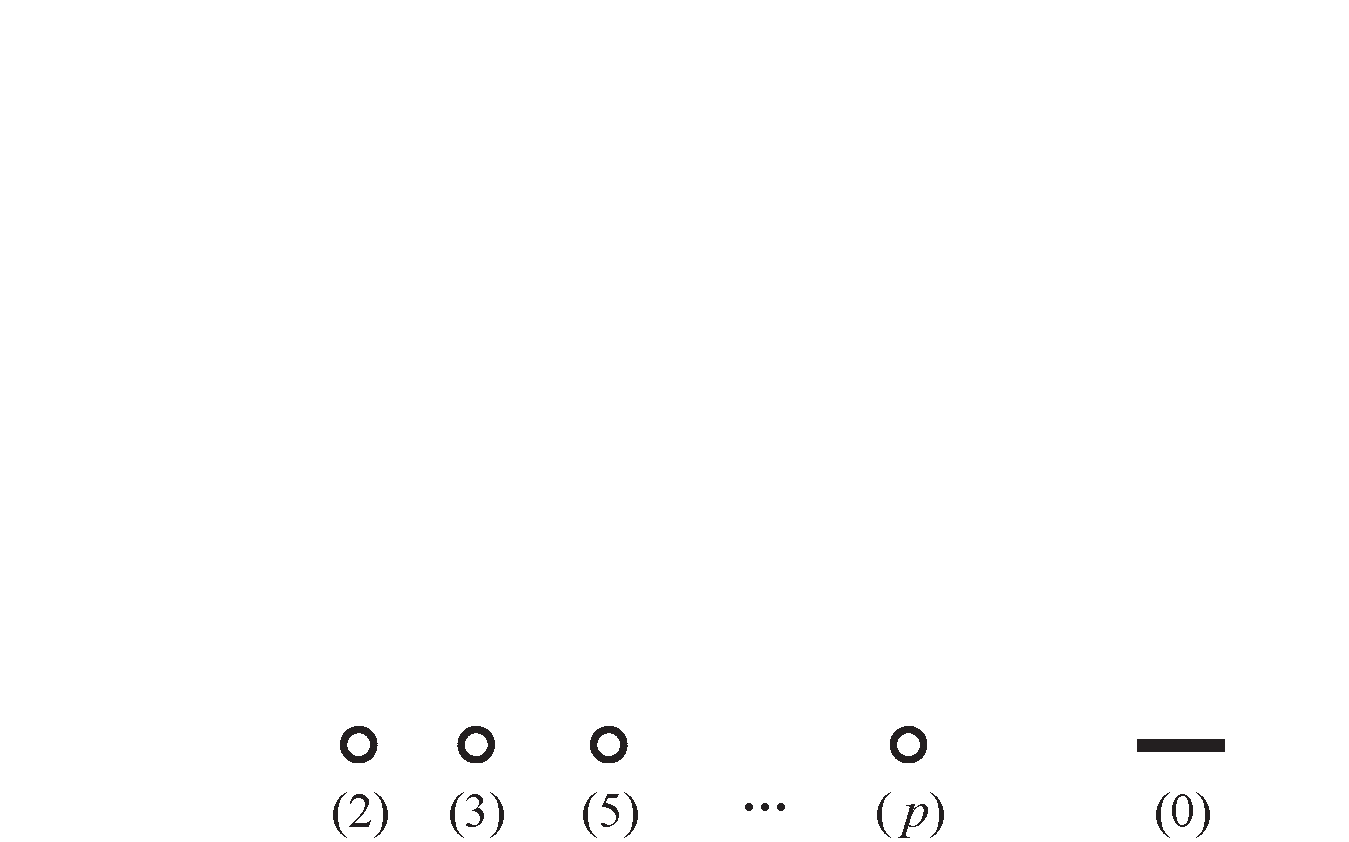
\includegraphics[width=3in]{SpecZ.pdf}
  \end{center}
  \par $\Spec(\mathbb{R})$ consists of one point $(0)$ since $(0)$ is the unique prime ideal in a field:
  \begin{center}
    \tikz\draw[black,ultra thick,fill=white] (0,0) circle (0.8ex);\\
    $(0)$
  \end{center}
  \par The prime ideals of $k[x]$ for $k$ a field are the ideals generated by irreducible polynomials and $(0)$ since $k[x]$ is a PID. Thus, $\Spec(\mathbb{C}[x])$ consists of prime ideals generated by linear polynomials $x - \alpha$ where $\alpha \in \mathbb{C}$ together with the point $(0)$ whose closure is all of $\Spec(\mathbb{C}[x])$, which we can visualize as a continuous line:
  \begin{center}
    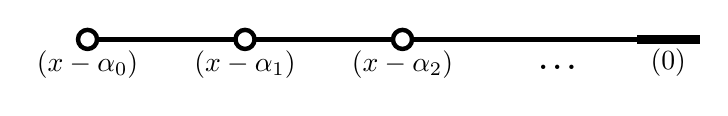
\begin{tikzpicture}
      \draw[ultra thick] (0,0) -- (7,0);
      \foreach \s in {0,1,2} {
        \draw[black,ultra thick,fill=white] (2*\s,0) circle (0.8ex) node[anchor=north] {$(x-\alpha_\s)$};
      }
      \node[anchor=north] at (6,-0.2) {\textbf{\dots}};
      \draw[black,ultra thick,fill=black] (7,-0.025) rectangle (7.75,0.025);
      \node[anchor=north] at (7.375,0) {$(0)$};
    \end{tikzpicture}
  \end{center}
  $\Spec(\mathbb{R}[x])$ consists of prime ideals generated by linear polynomials $x - a$ for $a \in \mathbb{R}$ and quadratic polynomials $(x - \beta)(x - \overline{\beta})$ for $\beta \in \mathbb{C}$, which we can visualize as a continuous line with two groups of closed points:
  \begin{center}
    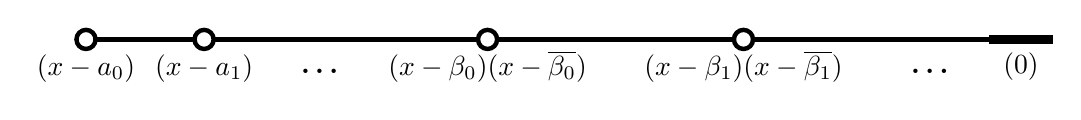
\begin{tikzpicture}
      \draw[ultra thick] (0,0) -- (12,0);
      \foreach \s in {0,1} {
        \draw[black,ultra thick,fill=white] (1.5*\s,0) circle (0.8ex) node[anchor=north] {$(x-a_\s)\vphantom{\overline{\beta}}$};
      }
      \node[anchor=north] at (3,-0.25) {\textbf{\dots}};
      \foreach \s in {0,1} {
        \draw[black,ultra thick,fill=white] (3.25*\s+5.1,0) circle (0.8ex) node[anchor=north] {$(x-\beta_\s)(x-\overline{\beta_\s})$};
      }
      \node[anchor=north] at (10.75,-0.25) {\textbf{\dots}};
      \draw[black,ultra thick,fill=black] (11.5,-0.025) rectangle (12.25,0.025);
      \node[anchor=north] at (11.875,0) {$(0)\vphantom{\overline{\beta}}$};
    \end{tikzpicture}
  \end{center}
  Note that $\Spec(\mathbb{C}[x])$ as a set is $\mathbb{C} \cup \{(0)\}$, and that $\Spec(\mathbb{R}[x])$ as a set is $\mathbb{H} \cup \{(0)\}$ where $\mathbb{H}$ is the upper half-plane $\{z \in \mathbb{C} \mid \operatorname{Im} z \ge 0\}$, but we chose to visualize $\Spec(\mathbb{C}[x])$ and $\Spec(\mathbb{R}[x])$ as above since they are one dimensional as rings.
  \par $\Spec(\mathbb{Z}[x])$ is visualized as a plane whose closed points are the maximal ideals of the form $(p,f)$ for $p$ a prime number and $f$ a polynomial irreducible mod $p$, with non-maximal prime ideals $(f)$ where $f$ is an irreducible polynomial, whose closure consist of all primes $(p,f)$, together with the point $(0)$ whose closure is everything: 
  \begin{equation*}
    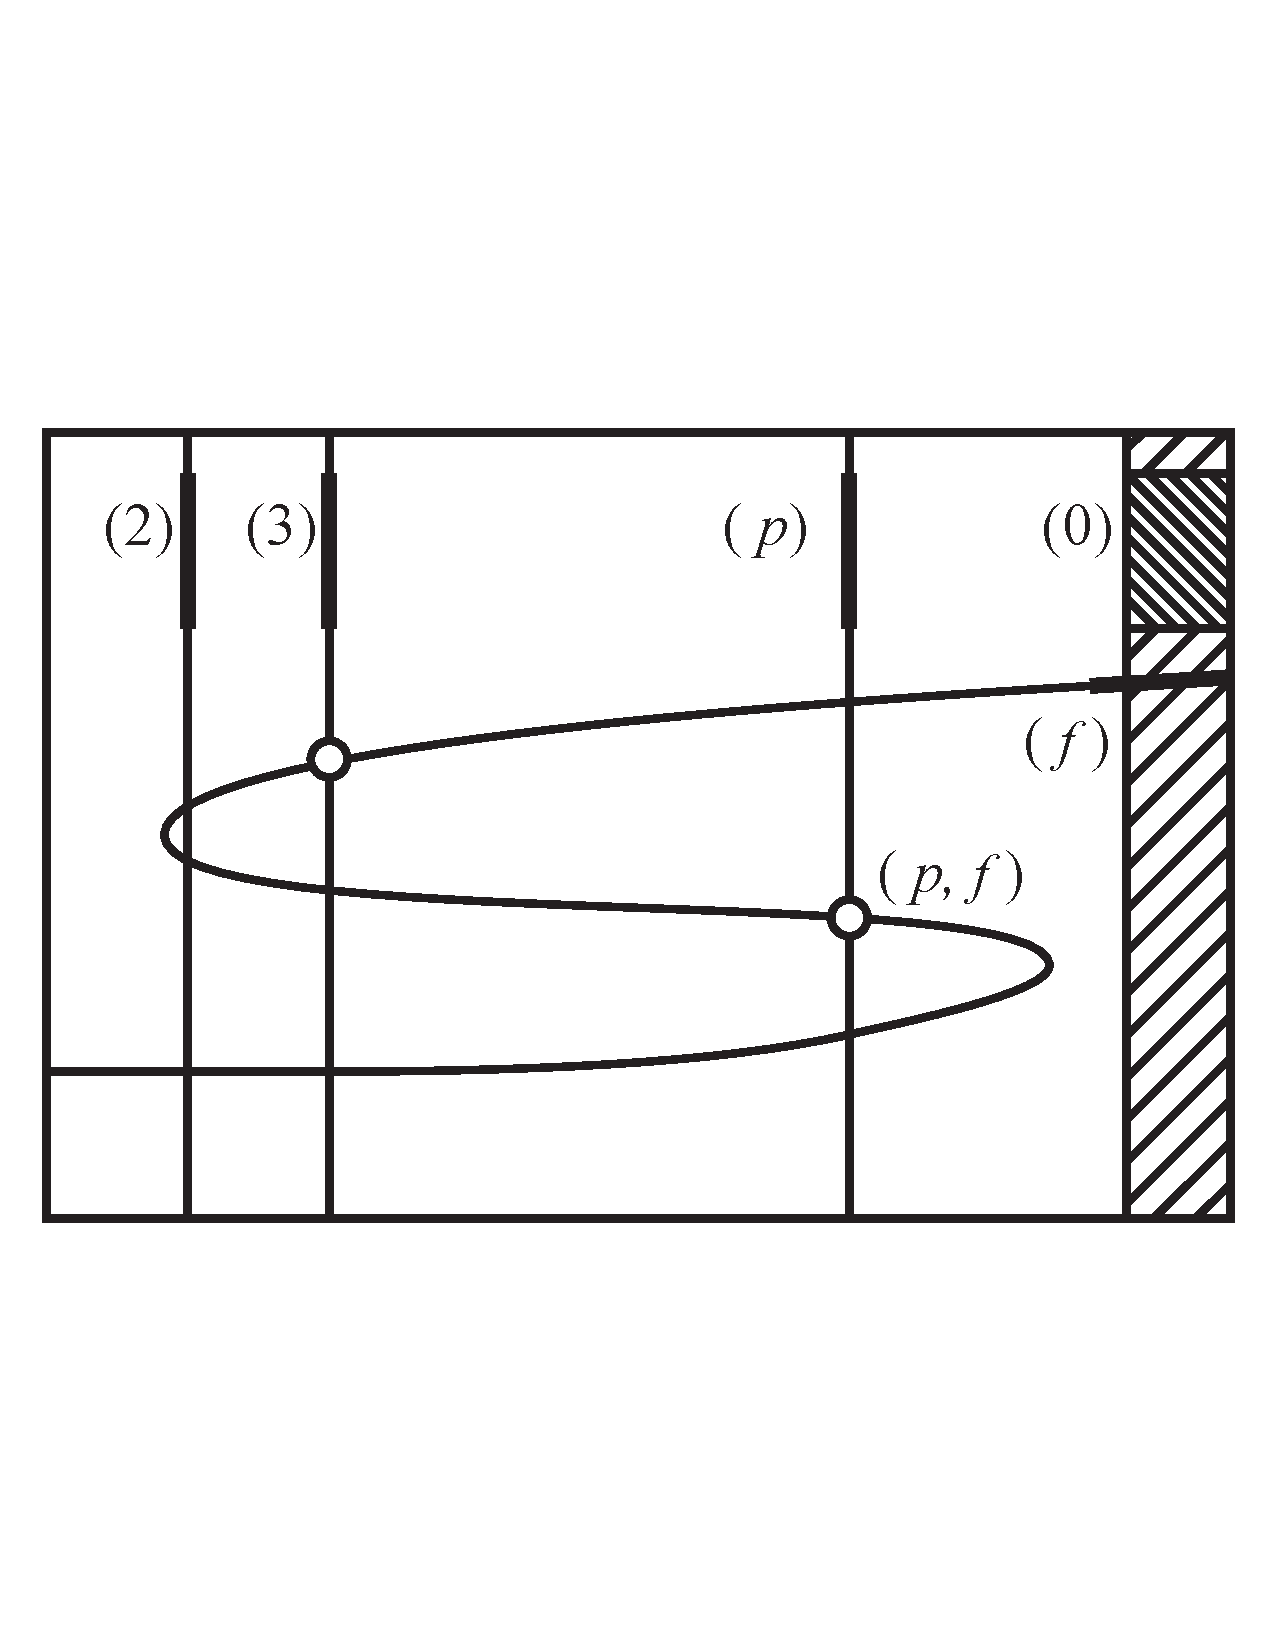
\includegraphics[width=3.5in]{SpecZx.pdf}
  \end{equation*}
  For completeness, we prove that these are all the prime ideals in $\mathbb{Z}[x]$. Let $\mathfrak{p} \subseteq \mathbb{Z}[x]$ be a prime ideal. If $\mathfrak{p}$ is $(0)$ or principal it is $(0)$ or $(f)$ for $f$ irreducible, so suppose not. We can then find $f_1,f_2 \in \mathfrak{p}$ with no common factor in $\mathbb{Z}[x]$.
  \par We claim $f_1,f_2$ do not share a factor in $\mathbb{Q}[x]$. For, if $f_1 = hg_1$ and $f_2 = hg_2$ with $h,g_1,g_2 \in \mathbb{Q}[x]$ and $\deg h \ge 1$. Write $h = ah_0$, $g_1 = b_1\gamma_1$, and $g_2 = b_2\gamma_2$ with $a,b_1,b_2 \in \mathbb{Q}$, and $h_0,\gamma_1,\gamma_2$ primitive elements of $\mathbb{Z}[x]$. By Exercise $\ref{exc:1.2}iv)$, $h_0\gamma_1$ and $h_0\gamma_2$ are primitive, hence $f_1 = hg_1 = (ab_1)(h_0\gamma_1) \in \mathbb{Z}[x]$ implies that $ab_1 \in \mathbb{Z}$, and similarly $ab_2 \in \mathbb{Z}$. Therefore $h_0 \mid f_1,f_2$, a contradiction.
  \par Now we claim $(f_1,f_2) \cap \mathbb{Z} \ne (0)$. $\mathbb{Q}[x]$ is a PID and $\gcd(f_1,f_2) = 1$, and so there exist $a,b \in \mathbb{Q}[x]$ such that $af_1 + bf_2 = 1$. If $c \in \mathbb{Z}$ is a common denominator of all the coefficients of $a$ and $b$ then $\mathbb{Z} \ni (ca)f_1 + (cb)f_2 = c$. Now since $\mathbb{Z}$ is a PID, and $(f_1,f_2 \cap \mathbb{Z}$ is a nonzero prime ideal, it is generated by $p$ prime in $\mathbb{Z}$.
\end{proof}

\begin{problem}\label{exc:1.17}
  For each $f \in A$, let $X_f$ denote the complement of $V(f)$ in $X = \Spec(A)$. The sets $X_f$ are open. Show that they form a basis of open sets for the Zariski topology, and that
  \begin{enumi}
    \item $X_f \cap X_g = X_{fg}$;
    \item $X_f = \emptyset \Leftrightarrow f$ is nilpotent;
    \item $X_f = X \Leftrightarrow f$ is a unit;
    \item $X_f = X_g \Leftrightarrow r\left( (f) \right) = r\left( (g) \right)$;
    \item $X$ is quasi-compact (that is, every open covering of $X$ has a finite sub-covering).
    \item More generally, each $X_f$ is quasi-compact.
    \item An open subset of $X$ is quasi-compact if and only if it is a finite union of sets $X_f$.
  \end{enumi}
  \par The sets $X_f$ are called \emph{basic open sets} of $X = \Spec(A)$.
\end{problem}
\begin{proof}[Proof of basis]
  Let $X \setminus V(E)$ be open; $\{X_f\}$ is a basis since by Exercise $\ref{exc:1.15}iii)$,
  \begin{equation*}
    X \setminus V(E) = X \setminus \bigcap_{f \in E} V(f) = \bigcup X_f.\qedhere
  \end{equation*}
\end{proof}
\begin{proof}[Proof of $i)$]
  $X_f \cap X_g = X \setminus (V(f) \cup V(g)) = X \setminus V(fg) = X_{fg}$ by Exercise $\ref{exc:1.15}iv)$.
\end{proof}
\begin{proof}[Proof of $ii)$]
  $X_f = \emptyset$ if and only if $f$ is contained in every prime ideal of $A$. But this holds if and only if $f \in \mathfrak{N}$ by Prop.~1.8, i.e., $f$ is nilpotent.
\end{proof}
\begin{proof}[Proof of $iii)$]
  $X_f = X$ if and only if $f$ is not contained in any prime ideal of $A$, which holds if and only if $f$ is a unit by Cor.~1.5.
\end{proof}
\begin{proof}[Proof of $iv)$]
  $\Leftarrow$. $X_f = X \setminus V(r(f)) = X \setminus V(r(g)) = X_g$ by Exercise $\ref{exc:1.15}i)$.
  \par $\Rightarrow$. $X_f = X_g$ implies $\mathfrak{p} \ni f$ if and only $\mathfrak{p} \ni g$, so $r(f) = r(g)$ by Prop.~1.14.
\end{proof}
\begin{proof}[Proof of $v)$]
  Since the $\{X_f\}$ form a basis by the above, any open cover of $X$ has a refinement of the form $\bigcup X_{f_\alpha}$. Thus, by Exercises $\ref{exc:1.15}ii)$ and $\ref{exc:1.15}iii)$,
  \begin{align*}
    X = \bigcup_{\alpha \in A} X_{f_\alpha} &\Leftrightarrow \emptyset = X \setminus \bigcup_{\alpha \in A} X_{f_\alpha} = \bigcap_{\alpha \in A} V(f_\alpha) = V\left( (f_\alpha)_{\alpha\in A} \right)\\
    &\Leftrightarrow 1 \in (f_\alpha)_{\alpha \in A}\\
    &\Leftrightarrow 1 = g_1f_1 + \cdots + g_mf_m\ \text{for some}\ g_i \in A, \{f_1,\ldots,f_m\} \subseteq \{f_\alpha\}\\
    &\Leftrightarrow \emptyset = V\left( (f_1,\ldots,f_{m}) \right) = \bigcap_{i=1}^m V(f_i)\\
    &\Leftrightarrow X = X_{f_1} \cup \cdots \cup X_{f_m}.\qedhere
  \end{align*}
\end{proof}
\begin{proof}[Proof of $vi)$]
  As in $v)$, any open cover of $X_f$ has a refinement of the form $\bigcup X_{f_\alpha}$. Now again, by Exercise $\ref{exc:1.15}iii)$,
  \begin{equation*}
    X_f \subseteq \bigcup_{\alpha \in A} X_{f_\alpha} \Leftrightarrow V(f) \supseteq \bigcap_{\alpha \in A} V(f_\alpha) = V\left( (f_\alpha)_{\alpha \in A} \right),
  \end{equation*}
  and so $f \in r\left( (f_\alpha)_{\alpha \in A} \right)$ by Prop.~1.14, i.e., $f^n = g_1f_1 + \cdots + g_mf_m$ for some $g_i \in A, \{f_1,\ldots,f_m\} \subseteq \{f_\alpha\}$. Then, since $V(f) = V(f^n)$ by Exercise $\ref{exc:1.15}i)$,
  \begin{equation*}
    V(f) \supseteq V\left( (f_1,\ldots,f_m) \right) = \bigcap_{i=1}^m V(f_i) \Leftrightarrow X_f \subseteq X_{f_1} \cup \cdots \cup X_{f_m}.\qedhere
  \end{equation*}
\end{proof}
\begin{proof}[Proof of $vii)$]
  $\Leftarrow$. Trivial since each $X_f$ is quasi-compact and open.
  \par $\Rightarrow$. $X$ can be written as a union of $X_f$ since $\{X_f\}$ is a basis, and we can find a finite subcover since $X$ is quasi-compact.
\end{proof}

\begin{problem}\label{exc:1.18}
  For psychological reasons it is sometimes convenient to denote a prime ideal of $A$ by a letter such as $x$ or $y$ when thinking of it as a point of $X = \Spec(A)$. When thinking of $x$ as a prime ideal of $A$, we denote it by $\mathfrak{p}_x$ (logically, of course, it is the same thing). Show that
  \begin{enumi}
    \item the set $\{x\}$ is closed (we say that $x$ is a ``closed point'') in $\Spec(A) \Leftrightarrow \mathfrak{p}_x$ is maximal;
    \item $\overline{\{x\}} = V(\mathfrak{p}_x)$;
    \item $y \in \overline{\{x\}} \Leftrightarrow \mathfrak{p}_x \subseteq \mathfrak{p}_y$;
    \item $X$ is a $T_0$-space (this means that if $x,y$ are distinct points of $X$, then either there is a neighborhood of $x$ which does not contain $y$, or else there is a neighborhood of $y$ which does not contain $x$).
  \end{enumi}
\end{problem}
\begin{proof}[Proof of $i)$]
  $\Leftarrow$. If $\mathfrak{p}_x$ is maximal, $V(\mathfrak{p}_x) = \{x\}$, and so $\{x\}$ is closed.
  \par $\Rightarrow$. If $\{x\}$ is closed, $\{x\} = V(\mathfrak{a})$ for some ideal $\mathfrak{a} \subsetneq A$ by Exercise $\ref{exc:1.15}i)$. By Cor.~1.4, there exists a maximal ideal $\mathfrak{m}$ containing $\mathfrak{a}$, and so $\mathfrak{m} \in V(\mathfrak{a}) = \{x\}$, and so $\mathfrak{p}_x = \mathfrak{m}$ is maximal.
\end{proof}
\begin{proof}[Proof of $ii)$]
  $\overline{\{x\}} \subseteq V(\mathfrak{p}_x)$ since $V(\mathfrak{p}_x) \ni \mathfrak{p}_x$. Conversely let $\mathfrak{p}_y \in V(\mathfrak{p}_x)$; we want to show that every $X_f \ni y$ intersects $\{x\}$. Suppose not; then there exists a basis element $X_f$ containing $y$ that does not contain $x$, and so $X \setminus X_f = V(f) \ni x$ but $V(f) \not\ni y$. In particular, $\mathfrak{p}_x \not\subseteq \mathfrak{p}_y$, and so $\mathfrak{p}_y \notin V(\mathfrak{p}_x)$, a contradiction.
\end{proof}
\begin{proof}[Proof of $iii)$]
  By $ii)$, $y \in \overline{\{x\}}$ if and only if $y \in V(\mathfrak{p}_x)$ if and only if $\mathfrak{p}_x \subseteq \mathfrak{p}_y$.
\end{proof}
\begin{proof}[Proof of $iv)$]
  Let $x,y\in X$ be distinct; then, say, $\mathfrak{p}_x \not\subseteq \mathfrak{p}_y$. So there exists $f \in \mathfrak{p}_x \setminus \mathfrak{p}_y$, and $\mathfrak{p}_y \in X_f$ but $\mathfrak{p}_x \notin X_f$.
\end{proof}

\begin{problem}\label{exc:1.19}
  A topological space $X$ is said to be \emph{irreducible} if $X \ne \emptyset$ and if every pair of non-empty open sets in $X$ intersect, or equivalently if every non-empty open set is dense in $X$. Show that $\Spec(A)$ is irreducible if and only if the nilradical of $A$ is a prime ideal.
\end{problem}
\begin{proof}
  $\Rightarrow$. Suppose $fg \in \mathfrak{N}$ but $f,g \notin \mathfrak{N}$. By Exercises $\ref{exc:1.17}i)$ and $\ref{exc:1.17}ii)$, $X_f,X_g$ are non-empty even though $X_f \cap X_g = X_{fg} = \emptyset$, hence $\Spec(A)$ is not irreducible.
  \par $\Leftarrow$. Suppose $\Spec(A)$ is not irreducible, and $U,V$ are non-empty disjoint open sets. Since $\{X_f\}$ is a basis by Exercise \ref{exc:1.17}, there exist $X_f \subseteq U,X_g \subseteq V$ such that $X_{fg} = X_f \cap X_g = \emptyset$ and so $fg \in \mathfrak{N}$ while $f,g \notin \mathfrak{N}$ by Exercises $\ref{exc:1.17}i)$ and $\ref{exc:1.17}ii)$. Thus, $\mathfrak{N}$ is not prime.
\end{proof}

\begin{problem}
  Let $X$ be a topological space.
  \begin{enumi}
  \item If $Y$ is an irreducible (Exercise $\hyperref[exc:1.19]{19}$) subspace of $X$, then the closure $\overline{Y}$ of $Y$ in $X$ is irreducible.
  \item Every irreducible subspace of $X$ is contained in a maximal irreducible subspace.
  \item The maximal irreducible subspaces of $X$ are closed and cover $X$. They are called the \emph{irreducible components} of $X$. What are the irreducible components of a Hausdorff space?
  \item If $A$ is a ring and $X = \Spec(A)$, then the irreducible components of $X$ are the closed sets $V(\mathfrak{p})$, where $\mathfrak{p}$ is a minimal prime ideal of $A$ (Exercise $\hyperref[exc:1.8]{8}$).
  \end{enumi}
\end{problem}
\begin{proof}[Proof of $i)$]
  Let $U,V \subseteq \overline{Y}$ open. Since $U$ is the neighborhood of some $x \in \overline{Y}$, we see that $U \cap Y \ne \emptyset$; similarly for $V \cap Y$. But since $U \cap Y,V \cap Y$ are open, $U \cap V \supseteq (U \cap Y) \cap (V \cap Y) \ne \emptyset$ by the irreducibility of $Y$.
\end{proof}
\begin{proof}[Proof of $ii)$]
  Let $Z$ be irreducible; we order the set $\Sigma$ of irreducible subspaces of $X$ containing $Z$ by inclusion. $\Sigma \ne \emptyset$ since $Z \in \Sigma$, and so by Zorn's lemma, it suffices to show any ascending chain $\{Y_\alpha\}_{\alpha \in A}$ has an upper bound $Y = \bigcup_{\alpha \in A} Y_\alpha$ in $\Sigma$. So let $U \cap Y,V \cap Y$ be non-empty opens in $Y$. Then, there exist $\alpha,\beta$ such that $U \cap Y_\alpha,V \cap Y_\beta$ are nonempty. Assuming without loss of generality that $\alpha \le \beta$, $U \cap Y_\beta \supseteq U \cap Y_\alpha$ is also nonempty, and $U \cap V \cap Y \supseteq U \cap V \cap Y_\beta \ne \emptyset$ by irreducibility of $Y_\beta$.
\end{proof}
\begin{proof}[Proof of $iii)$]
  Maximal irreducible subspaces $Y$ are closed since $\overline{Y}$ is also irreducible by $i)$, hence $Y = \overline{Y}$. They cover $X$ since $\{x\}$ is irreducible for any $x \in X$ (every nonempty open subset of $\{x\}$ contains $x$), and so $x$ is contained in some maximal irreducible subspace by $ii)$. 
  \par Suppose $X$is Hausdorff, and $Y \subseteq X$ is irreducible. If $Y$ is a one-point set, it is irreducible by above. If $Y \ni x,y$ for $x \ne y$, the Hausdorff axiom implies there exists open $U \ni x, V \ni y$ such that $U \cap V = \emptyset$, and so $Y$ is reducible. Thus the irreducible components are one-point sets.
\end{proof}
\begin{proof}[Proof of $iv)$]
  First, $X_f \cap V(\mathfrak{p}) \ne \emptyset$ if and only if $f \notin \mathfrak{q}$ for some prime ideal $\mathfrak{q} \supseteq \mathfrak{p}$, which occurs if and only if $f \notin \mathfrak{p}$.
  \par Now to show $V(\mathfrak{p})$ is irreducible, it suffices to show any non-empty basis elements $X_f \cap V(\mathfrak{p})$ and $X_g \cap V(\mathfrak{p})$ intersect. By the above, $f,g \notin \mathfrak{p}$, and by primeness, $fg \notin \mathfrak{p}$, hence
    $\mathfrak{p} \in X_{fg} \cap V(\mathfrak{p}) = X_f \cap X_g \cap V(\mathfrak{p})$.
    \par Conversely, suppose $Y \subseteq \Spec(A)$ is irreducible. $Y = V(r(\mathfrak{a}))$ for some ideal $\mathfrak{a} \subseteq A$ by Exercise $\ref{exc:1.15}i)$. Suppose $r(\mathfrak{a})$ is not prime, and $f,g \notin r(\mathfrak{a})$ such that $fg \in r(\mathfrak{a})$. There then exist $\mathfrak{p} \not\ni f$ and $\mathfrak{q} \not\ni g$ in $V(\mathfrak{a})$ by Prop.~$1.14$, and so by the first paragraph, $X_f \cap V(\mathfrak{p})$ and $X_g \cap V(\mathfrak{q})$ are non-empty. Thus $X_f \cap V(r(\mathfrak{a}))$ and $X_g \cap V(r(\mathfrak{a}))$ are non-empty. But by Exercise $\ref{exc:1.17}i)$, their intersection $X_{fg} \cap V(r(\mathfrak{a}))$ is empty since $fg \in r(\mathfrak{a})$ implies $fg \in \mathfrak{p}$ for any $\mathfrak{p} \in V(r(\mathfrak{a}))$, a contradiction.
    \par So, the irreducible subspaces of $X$ are of the form $V(\mathfrak{p})$ for $\mathfrak{p}$ prime. Moreover, $V(\mathfrak{p})$ is maximal among these subspaces if and only if $\mathfrak{p}$ is a minimal prime ideal, and so the irreducible components of $X$ are of the form $V(\mathfrak{p})$ for $\mathfrak{p}$ a minimal prime.
\end{proof}

\begin{problem}\label{exc:1.21}
  Let $\varphi\colon A \to B$ be a ring homomorphism. Let $X = \Spec(A)$ and $Y = \Spec(B)$. If $\mathfrak{q} \in Y$, then $\varphi^{-1}(\mathfrak{q})$ is a prime ideal of $A$, i.e., a point of $X$. Hence $\varphi$ induces a mapping $\varphi^*\colon Y \to X$. Show that
  \begin{enumi}
    \item If $f \in A$ then $\varphi^{*-1}(X_f) = Y_{\varphi(f)}$, hence that $\varphi^*$ is continuous.
    \item If $\mathfrak{a}$ is an ideal of $A$, then $\varphi^{*-1}(V(\mathfrak{a})) = V(\mathfrak{a}^e)$.
    \item If $\mathfrak{b}$ is an ideal of $B$, then $\overline{\varphi^*( V(\mathfrak{b}))} = V(\mathfrak{b}^c)$.
    \item If $\varphi$ is surjective, then $\varphi^*$ is a homeomorphism of $Y$ onto the closed subset $V( \Ker(\varphi) )$ of $X$. (In particular, $\Spec(A)$ and $\Spec(A/\mathfrak{N})$ (where $\mathfrak{N}$ is the nilradical of $A$) are naturally homeomorphic.)
    \item If $\varphi$ is injective, then $\varphi^*(Y)$ is dense in $X$. More precisely, $\varphi^*(Y)$ is dense in $X \Leftrightarrow \Ker(\varphi) \subseteq \mathfrak{N}$.
    \item Let $\psi\colon B \to C$ be another ring homomorphism. Then $(\psi \circ \varphi)^* = \varphi^* \circ \psi^*$.
    \item Let $A$ be an integral domain with just one non-zero prime ideal $\mathfrak{p}$, and let $K$ be the field of fractions of $A$. Let $B = (A/\mathfrak{p}) \times K$. Define $\varphi\colon A \to B$ by $\varphi(x) = (\overline{x},x)$, where $\overline{x}$ is the image of $x$ in $A/\mathfrak{p}$. Show that $\varphi^*$ is bijective but not a homeomorphism.
  \end{enumi}
\end{problem}
\begin{proof}[Proof of $i)$]
  $\varphi^{*-1}(X_f) = \{\mathfrak{q} \in Y \mid f \notin \mathfrak{q}^c\} = \{\mathfrak{q} \in Y \mid \varphi(f) \notin \mathfrak{q}\} = Y_{\varphi(f)}$, so $\varphi^*$ is continuous since the inverse images of basis elements are basis elements.
\end{proof}
\begin{proof}[Proof of $ii)$]
  Using $i)$ and Exercise $\ref{exc:1.15}iii)$, we have
  \begin{align*}
    \varphi^{*-1}\left(V(\mathfrak{a})\right) &= \varphi^{*-1}\left( V\left( \bigcup_{x \in \mathfrak{a}} \{x\} \right) \right) = \varphi^{*-1}\left( \bigcap_{x \in \mathfrak{a}}V(x) \right)\\
    &= \bigcap_{x \in \mathfrak{a}}\varphi^{*-1}\left( V(x) \right) = \bigcap_{x \in \mathfrak{a}}\varphi^{*-1}\left( X \setminus X_x \right) = \bigcap_{x \in \mathfrak{a}}\left(Y \setminus \varphi^{*-1}\left(X_x\right)\right)\\
    &= \bigcap_{x \in \mathfrak{a}}\left(Y \setminus Y_{\varphi(x)}\right) = \bigcap_{x \in \mathfrak{a}} V(\varphi(x)) = V(\mathfrak{a}^e).\qedhere
  \end{align*}
\end{proof}
\begin{proof}[Proof of $iii)$]
  First, we have $\overline{\varphi^*\left( V(\mathfrak{b}) \right)} \subseteq V(\mathfrak{b}^c)$ since
  \begin{equation*}
    \varphi^*( V(\mathfrak{b})) = \{\mathfrak{q}^c \in X \mid \mathfrak{q} \in Y,\ \mathfrak{b} \subseteq \mathfrak{q}\} \subseteq \{\mathfrak{p} \in X \mid \mathfrak{b}^c \subseteq \mathfrak{p}\} = V(\mathfrak{b}^c).
  \end{equation*}
  Conversely, suppose $\mathfrak{p} \in V(\mathfrak{b}^c)$; to show $\mathfrak{p} \in \overline{\varphi^*\left( V(\mathfrak{b}) \right)}$, it suffices to show every $X_f \ni \mathfrak{p}$ intersects $\varphi^*\left( V(\mathfrak{b}) \right)$. Now $X_f \ni \mathfrak{p}$ implies $f \notin \mathfrak{p}$, hence $f \notin r(\mathfrak{b}^c) = r(\mathfrak{b})^c$ by Exercise $1.18$ in the text. Thus, $\varphi(f) \notin r(\mathfrak{b})$, and so there exists $\mathfrak{q} \in V(\mathfrak{b})$ such that $\varphi(f) \notin \mathfrak{q}$ by Prop.~1.14. Then, $f \notin \mathfrak{q}^c$, and so $\mathfrak{q}^c \in X_f$, i.e., $\varphi^*(V(\mathfrak{b})) \cap X_f \ne \emptyset$.
\end{proof}
\begin{proof}[Proof of $iv)$]
  If $\varphi$ is surjective, we have a bijection between primes containing $\Ker\varphi$ in $A$ and primes in $B$ by Prop.~1.1. We claim this induces a homeomorphism $\varphi^*\colon Y \to V(\Ker\varphi)$; since it is continuous by $i)$, it remains to show it is closed. By $iii)$, we know $\varphi^*(V(\mathfrak{b})) \subseteq V(\mathfrak{b}^c)$ for any ideal $\mathfrak{b} \subseteq B$. If $\mathfrak{p} \in V(\mathfrak{b}^c)$ then $\varphi(\mathfrak{p}) \supseteq \varphi(\mathfrak{b}^c) = \mathfrak{b}$ by surjectivity of $\varphi$, and so $\varphi(\mathfrak{p}) \in V(\mathfrak{b})$. But then $\mathfrak{p} = \varphi^*(\varphi(\mathfrak{p})) \in \varphi^*(V(\mathfrak{b}))$.
  \par Finally, $A \to A/\mathfrak{N}$ is surjective, hence $\Spec(A/\mathfrak{N})$ is homeomorphic to $V(\mathfrak{N})$. Since $V(\mathfrak{N})=\Spec(A)$ by Prop.~1.1 and Prop.~1.8, we have that $\Spec(A)$ and $\Spec(A/\mathfrak{N})$ are homeomorphic.
\end{proof}
\begin{proof}[Proof of $v)$]
  We see by $iii)$ that $X \supseteq \overline{\varphi^*(Y)} = \overline{\varphi^*(V(0))} = V(0^c) = V(\Ker(\varphi))$, so $\varphi^*(Y)$ dense in $X$ if and only if $V(\Ker(\varphi)) = X$ if and only if $\Ker(\varphi) \subseteq \mathfrak{N}$ by Prop.~1.8. In particular, if $\varphi$ injective, $\Ker(\varphi) = 0 \subseteq \mathfrak{N}$, so $\varphi^*(Y)$ is dense in $X$.
\end{proof}
\begin{proof}[Proof of $vi)$]
  $(\psi \circ \varphi)^*(\mathfrak{r}) = (\psi \circ \varphi)^{-1}(\mathfrak{r}) = \varphi^{-1}(\psi^{-1}(\mathfrak{r})) = \varphi^*(\psi^*(\mathfrak{r}))$ for every $\mathfrak{r} \in \Spec(C)$, hence $(\psi \circ \varphi)^* = \varphi^* \circ \psi^*$.
\end{proof}
\begin{proof}[Proof of $vii)$]
  $A/\mathfrak{p}$ is a field since $\mathfrak{p}$ is maximal in $A$. The ideals $\mathfrak{q}_1 = \{(\overline{x},0) \in B\}$ and $\mathfrak{q}_2 = \{(0,x) \in B\}$ are maximal, since $B/\mathfrak{q}_1 \cong K$ and $B/\mathfrak{q}_2 \cong A/\mathfrak{p}$. If $\mathfrak{q}$ is another prime of $B$, then $\mathfrak{q}_1\mathfrak{q}_2 = 0 \subseteq \mathfrak{q}$, hence $\mathfrak{q}_1 \subseteq \mathfrak{q}$ or $\mathfrak{q}_2 \subseteq \mathfrak{q}$, which implies $\mathfrak{q} = \mathfrak{q}_1$ or $\mathfrak{q}_2$ by maximality, and so $\Spec(B) = \{\mathfrak{q}_1,\mathfrak{q}_2\}$. Since $\varphi^*(\mathfrak{q}_1) = 0$ and $\varphi^*(\mathfrak{q}_2) = \mathfrak{p}$, $\varphi^*$ is bijective. But $\varphi^*$ is not a homeomorphism since $\Spec(A)$ has a non-closed point while $\Spec(B)$ does not. 
\end{proof}

\begin{problem}
  Let $A = \prod_{i=1}^n A_i$ be the direct product of rings $A_i$. Show that $\Spec(A)$ is the disjoint union of open (and closed) subspaces $X_i$, where $X_i$ is canonically homeomorphic with $\Spec(A_i)$.
  \par Conversely, let $A$ be any ring. Show that the following statements are equivalent:
  \begin{enumi}
    \item $X = \Spec(A)$ is disconnected.
    \item $A \cong A_1 \times A_2$ where neither of the rings $A_1,A_2$ is the zero ring.
    \item $A$ contains an idempotent $\ne 0,1$.
  \end{enumi}
  \par In particular, the spectrum of a local ring is always connected (Exercise $\hyperref[exc:1.12]{12}$).
\end{problem}
\begin{proof}[Proof of first statement]
  Consider the projection map $\pi_i\colon A \to A_i$. $\pi_i$ is surjective, hence induces a homeomorphism $\pi_i^*\colon\Spec A_i \isoto V(\Ker(\pi_i))$ by Exercise $\ref{exc:1.21}iv)$. Letting $X_i \coloneqq V(\Ker(\pi_i))$, we have $\Spec(A) \supseteq \bigcup_{i=1}^n X_i$. By Exercise \ref{exc:1.15}, we have
  \begin{gather*}
    \bigcup_{i=1}^n X_i = V\left(\bigcap_{i=1}^n\Ker(\pi_i)\right) = V(0) = \Spec(A),\\
    X_i \cap X_j = V( \Ker(\pi_i) + \Ker(\pi_j)) = V(1) = \emptyset,
  \end{gather*}
  and so $\Spec(A) = \coprod_{i=1}^n X_i$, where each $X_i$ is closed in $\Spec(A)$ hence open since $\Spec(A) \setminus X_i$ is a finite union of closed subsets of $\Spec(A)$.
\end{proof}
\begin{proof}[Proof of second statement]
  $(ii) \Rightarrow (i)$. This is the first statement.
  \par $(i) \Rightarrow (iii)$. Suppose $X = X_1 \amalg X_2$, where $X_1 = V(\mathfrak{a}_1)$, $X_2 = V(\mathfrak{a}_2)$ for ideals $\mathfrak{a}_i \subseteq A$. By Exercise $\ref{exc:1.15}$, $V(1) = \emptyset = V(\mathfrak{a}_1 + \mathfrak{a}_2)$ implies $\sqrt{\mathfrak{a}_1 + \mathfrak{a}_2} = A$, so by Exercise $1.13iv)$ in the text, $\mathfrak{a}_1 + \mathfrak{a}_2 = 1$, i.e., $x_1 + x_2 = 1$ for some $x_1 \in \mathfrak{a}_1,x_2\in\mathfrak{a}_2$. Now $X = V(0) = V(\mathfrak{a}_1\cdot\mathfrak{a}_2)$ implies $\mathfrak{a}_1\mathfrak{a}_2 \subseteq \sqrt{0}$, and so $(x_1x_2)^m = 0$ for some $m$. Thus, define
  \begin{equation*}
    1 = (x_1 + x_2)^{2m} = \underbrace{x_1^{2m} + \cdots + \binom{2m}{m+1} x_1^{m+1}x_2^{m-1}}_{e_1} + \underbrace{\binom{2m}{m}x_1^mx_2^m + \cdots + x_2^{2m}}_{e_2}
  \end{equation*}
  We have $e_1e_2 = 0$ since each term in the product contains $(x_1x_2)^m$. Then, $e_1 = e_1(e_1 + e_2) = e_1^2$ and so $A$ contains an idempotent $\ne 0,1$.
  \par $(iii) \Rightarrow (ii)$. Let $A_1 = A/(e)$ and $A_2 = A/(1-e)$, where $e \ne0,1$ is idempotent. $A_1 \ne 0$ since if $e \in A^\times$, $1 = ee^{-1} = e^2e^{-1} = e$, a contradiction; similarly, $A_2 \ne 0$ since if $1-e \in A^\times$, $1 = (1-e)(1-e)^{-1} = (1-e)^2(1-e)^{-1} = 1-e$, implying $e=0$. Thus, $A \to A_1 \times A_2$ is an isomorphism by Prop.~1.10 since $(e) + (1-e) = (1)$ and $(e) \cap (1-e) = (e(1-e)) = (e-e^2) = (0)$.
\end{proof}

\begin{problem}\label{exc:1.23}
  Let $A$ be a Boolean ring (Exercise $\hyperref[exc:1.11]{11}$), and let $X = \Spec(A)$.
  \begin{enumi}
    \item For each $f \in A$, the set $X_f$ (Exercise $\hyperref[exc:1.17]{17}$) is both open and closed in $X$.
    \item Let $f_1,\ldots,f_n \in A$. Show that $X_{f_1} \cup \cdots \cup X_{f_n} = X_f$ for some $f \in A$.
    \item The sets $X_f$ are the only subsets of $X$ which are both open and closed.
    \item $X$ is a compact Hausdorff space.
  \end{enumi}
\end{problem}
\begin{proof}[Proof of $i)$]
  $X_f$ is open by definition. Now if $\mathfrak{p} \in X$, then $f(1-f) = 0$ implies either $f \in \mathfrak{p}$ or $(1-f) \in \mathfrak{p}$, exclusively, hence $X_f = V(1-f)$ is also closed.
\end{proof}
\begin{proof}[Proof of $ii)$]
  By $i)$, $X_{f_1} \cup \cdots \cup X_{f_n} = V(\mathfrak{a})$ for some ideal $\mathfrak{a} \subseteq A$. By Exercise $\ref{exc:1.11}iii)$, $\mathfrak{a} = (g)$ for some $g \in A$, so letting $f = 1-g$, $X_f = V(g) = X_{f_1} \cup \cdots \cup X_{f_n}$ by $i)$.
\end{proof}
\begin{proof}[Proof of $iii)$]
  If $Y \subseteq X$ is closed, it is quasi-compact since $X$ is by Exercise $\ref{exc:1.17}v)$. If $Y$ is also open, $Y = X_{f_1} \cup \cdots \cup X_{f_n}$ for some $f_i$ by Exercise $\ref{exc:1.17}vii)$. By $ii)$, $Y = X_f$ for some $f$.
\end{proof}
\begin{proof}[Proof of $iv)$]
  $X$ is quasi-compact by Exercise $\ref{exc:1.17}v)$. Suppose $\mathfrak{p} \ne \mathfrak{q}$. By Exercise $\ref{exc:1.11}iii)$, $\mathfrak{p} = (f)$ for some $f \in A$, and $f \notin \mathfrak{q}$. By the argument in $i)$, $\mathfrak{p} \in V(f) = X_{1-f}$ while $\mathfrak{q} \in X_f$, hence $X$ is Hausdorff.
\end{proof}

\begin{problem}
  Let $L$ be a lattice, in which the $\sup$ and $\inf$ of two elements $a,b$ are denoted by $a \lor b$ and $a \land b$ respectively. $L$ is a \emph{Boolean lattice} (or \emph{Boolean algebra}) if
  \begin{enumi}
    \item $L$ has a least element and a greatest element (denoted by $0,1$ respectively).
    \item Each of $\lor$, $\land$ is distributive over the other.
    \item Each $a \in L$ has a unique ``complement'' $a' \in L$ such that $a \lor a' = 1$ and $a \land a' = 0$.
  \end{enumi}
  (For example, the set of all subsets of a set, ordered by inclusion, is a Boolean lattice).
  \par Let $L$ be a Boolean lattice. Define addition and multiplication in $L$ by the rules
  \begin{equation*}
    a + b = (a \land b') \lor (a' \land b), \qquad ab = a \land b.
  \end{equation*}
  Verify in this way $L$ becomes a Boolean ring, say $A(L)$.
  \par Conversely, starting from a Boolean ring $A$, define an ordering on $A$ as follows: $a \le b$ means that $a = ab$. Show that, with respect to this ordering, $A$ is a Boolean lattice. [The $\sup$ and $\inf$ are given by $a \lor b = a + b + ab$ and $a \land b = ab$, and the complement by $a' = 1 - a$.] In this way we obtain a one-to-one correspondence between (isomorphism classes of) Boolean rings and (isomorphism classes of) Boolean lattices.
\end{problem}
\begin{proof}[Proof that $A(L)$ is a Boolean ring]
  $0 \land 0 = 0$ implies $0' = 0$. So, $L$ is an abelian group with respect to addition since it is abelian by definition of $\sup,\inf$, has inverses by $iii)$, and has identity $0$ since $a + 0 = (a \land 0') \lor (a' \land 0) = 0 \lor 0 = 0$ by definition of $\sup,\inf$. Multiplication is associative by definition of $\inf$, distributes over addition by $ii)$, is commutative by definition of $\inf$, and has identity $1$ since $1a = 1 \lor a = a$ by definition of $\sup$.
  \par $L$ is a Boolean ring since $x^2 = x \land x = x$ for all $x \in L$ by definition of $\inf$.
\end{proof}
\begin{proof}[Proof that $L(A)$ is a Boolean lattice]
  $A$ is a poset under $\le$ since $a \le a$ is the condition $a = a^2$, $a \le b$ and $b \le a$ imply both $a = ab$ and $b = ab$ so $a = b$, and since $a \le b$ and $b \le c$ imply both $a = ab$ and $b = bc$ so $a = ac$, i.e., $a \le c$. $\sup,\inf$ define upper and lower bounds for two elements in $A$, respectively, and so it remains to show they are least upper and greatest lowest bounds, respectively. So suppose $c < \sup\{a,b\}$ but both $a \le c$ and $b \le c$. Then, $a = ac$ and $b = bc$, so $\sup\{a,b\} = a + b + ab = ac + bc + abc = \sup\{a,b\}c$ implies $c = 1$, a contradiction. Suppose $1 \ne \inf\{a,b\} < c$ but both $c \le a$ and $c \le a$; note the $\inf\{a,b\} = 1$ case is trivial since this implies $a=b=1$. Then, $c = ac$ and $c = bc$, so $\inf\{a,b\}c = abc = c$ implies $c = 0$, a contradiction.
  \par $i)$. $0$ is the least element since $a \land 0 = 0$ for any $a \in A$. $1$ is the greatest element since $a \lor 1 = a + 1 + a = 1$ for any $a \in A$ by Exercise $\ref{exc:1.11}i)$.
  \par $ii)$. Using Exercise $\ref{exc:1.11}i)$,
  \begin{align*}
    a \lor (a \land b) &= a + ab + a^2b = a + ab + ab = a,\\
    a \land (a \lor b) &= a(a \lor b) = a(a + b + ab) = a^2 + ab + a^2b = a + ab + ab = a.
  \end{align*}
  \par $iii)$. We see $a \land a' = aa' = a(1-a) = 1$ and $a \lor a' = a + (1-a) + a(1-a) = 1 + 1 = 0$ by Exercise $\ref{exc:1.11}i)$, and $a'$ is unique since multiplicative inverses are unique.
\end{proof}
\begin{proof}[Proof of correspondence]
  The operations $L \mapsto A(L)$ and $A \mapsto L(A)$ are bijections on sets, and so to show we have a bijection on isomorphism classes, it suffices to show that the lattice structure on $L$ and $L(A(L))$ are the same, and similarly the ring structure on $A$ and $A(L(A))$ are the same.
  \par If $L$ is a Boolean lattice, then $A(L)$ has $ab = a \land b$, and so $L(A(L))$ has $a \leqslant b$ defined by $a = ab = a \land b$. Now $a \leqslant b$ if and only if $a = a \land b$ if and only if $a \le b$.
  \par If $A$ is a Boolean ring, then $L(A)$ has $a \lor b = a + b + ab$ and $a \land b = ab$. Letting $\oplus,\otimes$ be the operations on $A(L(A))$, $a \otimes b = a \land b = ab$, and using Exercise $\ref{exc:1.11}i)$,
  \begin{align*}
    a \oplus b &= (a \land b') \lor (a' \land b) = ab' \lor a'b = ab' + a'b + aa'bb'\\
    &= a(1-b) + (1-a)b + a(1-a)b(1-b)\\
    &= a - ab + b - ab + (a-a^2)(b-b^2) = a + b.\qedhere
  \end{align*}
\end{proof}

\begin{problem}
  From the last two exercises deduce Stone's theorem, that every Boolean lattice is isomorphic to the lattice of open-and-closed subsets of some compact Hausdorff topological space.
\end{problem}
\begin{proof}
  Consider the lattice $\LL$ of open-and-closed subsets of $\Spec (A(L))$ as a poset under inclusion of subsets $\subseteq$. By Exercise $\ref{exc:1.23}iv)$, $\Spec(A(L))$ is compact Hausdorff. We claim that the map $\varphi\colon L \to \LL$ sending $f \mapsto X_f$ is an isomorphism of lattices.
  \par We first show $\varphi$ is a bijection. By Exercise $\ref{exc:1.23}iii)$, $\varphi$ is surjective. $\varphi$ is injective since if $X_f = X_g$, then
  \begin{equation*}
    \emptyset = X_{1-f} \cap X_f = X_{1-f} \cap X_g = X_{(1-f)g}
  \end{equation*}
  using Exercises $\ref{exc:1.17}i)$ and $\ref{exc:1.23}i)$, hence by Exercise $\ref{exc:1.17}ii)$, $(1-f)g \in \mathfrak{N}$. So, $\left((1-f)g\right)^m = 0$ for some $m$, and $(1-f)g = 0$ since $A(L)$ is Boolean. Thus, $g = fg$. We can show $f = fg$ using the same argument, and so $g \le f$ and $f \le g$ imply $f = g$.
  \par We now know the map $\varphi^{-1}$ mapping $X_f \mapsto f$ is well-defined, and so by \cite[Thm.~2.3]{BS81}, it suffices to show $\varphi,\varphi^{-1}$ are both order-preserving. Using Exercise $\ref{exc:1.17}i)$,
  \begin{equation*}
    f \le g \Leftrightarrow f = fg \Leftrightarrow X_f = X_f \cap X_g \Leftrightarrow X_f \subseteq X_g.\qedhere
  \end{equation*}
\end{proof}

\begin{problem}\label{exc:1.26}
  Let $A$ be a ring. The subspace of $\Spec(A)$ consisting of the \emph{maximal} ideals of $A$, with the induced topology, is called the \emph{maximal spectrum} of $A$ and is denoted by $\Max(A)$. For arbitrary commutative rings it does not have the nice functorial properties of $\Spec(A)$ (see Exercise \hyperref[exc:1.21]{$21$}), because the inverse image of a maximal ideal under a ring homomorphism need not be maximal.
  \par Let $X$ be a compact Hausdorff space and let $C(X)$ denote the ring of all real-valued continuous functions on $X$ (add and multiply functions by adding and multiplying their values). For each $x \in X$, let $\mathfrak{m}_x$ be the set of all $f \in C(X)$ such that $f(x) = 0$. The ideal $\mathfrak{m}_x$ is maxmal, because it is the kernel of the (surjective) homomorphism $C(X) \to \mathbb{R}$ which takes $f$ to $f(x)$. If $\tilde{X}$ denotes $\Max(C(X))$, we have therefore defined a mapping $\mu\colon X \to \tilde{X}$, namely $x \mapsto \mathfrak{m}_x$.
  \par We shall show that $\mu$ is a homeomorphism of $X$ onto $\tilde{X}$.
  \begin{enumi}
    \item Let $\mathfrak{m}$ be any maximal ideal of $C(X)$, and let $V = V(\mathfrak{m})$ be the set of common zeros of the functions in $\mathfrak{m}$: that is,
      \begin{equation*}
        V = \{x \in X : f(x) = 0~\text{for all}~f \in \mathfrak{m}\}.
      \end{equation*}
      Suppose that $V$ is empty. Then for each $x \in X$ there exists $f_x \in \mathfrak{m}$ such that $f_x(x) \ne 0$. Since $f_x$ is continuous, there is an open neighborhood $U_x$ of $x$ in $X$ on which $f_x$ does not vanish. By compactness a finite number of neighborhoods, say $U_{x_1},\ldots,U_{x_n}$, cover $X$. Let
      \begin{equation*}
        f = f_{x_1}^2 + \cdots + f_{x_n}^2.
      \end{equation*}
      Then $f$ does not vanish at any point of $X$, hence is a unit in $C(X)$. But this contradicts $f \in \mathfrak{m}$, hence $V$ is not empty.
      \par \hspace{1.25em} Let $x$ be a point of $V$. Then $\mathfrak{m} \subseteq \mathfrak{m}_x$, hence $\mathfrak{m} = \mathfrak{m}_x$ because $\mathfrak{m}$ is maximal. Hence $\mu$ is surjective.
    \item By Urysohn's lemma (this is the only non-trivial fact required in the argument) the continuous functions separate the points of $X$. Hence $x \ne y \Rightarrow \mathfrak{m}_x \ne \mathfrak{m}_y$, and therefore $\mu$ is injective.
    \item Let $f \in C(X)$; let
      \begin{equation*}
        U_f = \{x \in X : f(x) \ne 0\}
      \end{equation*}
      and let
      \begin{equation*}
        \tilde{U}_f = \{\mathfrak{m} \in \tilde{X} : f \notin \mathfrak{m}\}
      \end{equation*}
      Show that $\mu(U_f) = \tilde{U}_f$. The open sets $U_f$ (resp.~$\tilde{U}_f$) form a basis of the topology of $X$ (resp.~$\tilde{X}$) and therefore $\mu$ is a homeomorphism.
      \par Thus $X$ can be reconstructed from the ring of functions $C(X)$.
  \end{enumi}
\end{problem}
\begin{proof}[Proof of $i)$]
  Let $\mathfrak{m} \in \tilde{X}$, and let $V = \{x \in X : f(x) = 0~\text{for all}~f \in \mathfrak{m}\}$. If $V$ is empty, then for each $x$ there is $f_x \in \mathfrak{m}$ such that $f_x(x) \ne 0$; since each $f_x$ is continuous, there is an open neighborhood $U_x \ni x$ in $X$ such that $f_x \ne 0$ on $U_x$. Since $X$ is compact, finitely many $U_x$ say $U_{x_1},\ldots,U_{x_n}$ cover $X$. Letting $f = \sum f_{x_i}^2$, we see $f \ne 0$ anywhere on $X$, hence $f \in C(X)^\times$ with inverse $1/f$. But this contradicts $f \in \mathfrak{m}$, hence $V \ne \emptyset$. Now if $x \in V$, then $\mathfrak{m} \subseteq \mathfrak{m}_x$, and this is moreover an equality since $\mathfrak{m}$ is maximal. Thus, $\mu(x) = \mathfrak{m}$ and so $\mu$ is surjective.
\end{proof}
\begin{proof}[Proof of $ii)$]
  Since $X$ is compact Hausdorff, it is normal \cite[Thm.~32.3]{Mun00}, and so by Urysohn's lemma \cite[Thm.~33.1]{Mun00}, if $x \ne y$ there exists $f_x$ such that $f_x(x) = 0$ while $f_x(y) = 1$; similarly, there exists $f_y$ such that $f_y(x) = 1$ while $f_y(y) = 0$. Then, $f_x \in \mathfrak{m}_x \setminus \mathfrak{m}_y$ and $f_y \in \mathfrak{m}_y \setminus \mathfrak{m}_x$, hence $\mathfrak{m}_x \ne \mathfrak{m}_y$, and so $\mu$ is injective.
\end{proof}
\begin{proof}[Proof of $iii)$]
  By $i)$, every $\mathfrak{m} \in \tilde{X}$ is of the form $\mathfrak{m}_x$ for some $x \in X$, so
  \begin{equation*}
    \mu(U_f) = \{\mathfrak{m}_x \in \tilde{X} : f(x) \ne 0\} = \{\mathfrak{m}_x \in \tilde{X} : f \notin \mathfrak{m}_x\} = \tilde{U}_f.
  \end{equation*}
  $U_f$ is open since $f$ is continuous. Now if $x \in U \subseteq X$, then since $X$ is normal as in $ii)$, there is a neighborhood $V \ni x$ such that $\bar{V} \subseteq U$ \cite[Lem.~$31.1(b)$]{Mun00}. By Urysohn's lemma, there exists $f \in C(X)$ such that $f = 1$ on $\bar{V}$ and $f = 0$ on $X \setminus U$. So, $x \in U_f \subseteq U$, hence the $U_f$ are a basis for $X$.
  \par The $\tilde{U}_f$ are open since $\tilde{X}$ has the subspace topology induced from $\Spec(C(X))$, and $\tilde{U}_f = (\Spec(C(X)))_f \cap \tilde{X}$ where $(\Spec(C(X)))_f$ is as in Exercise \ref{exc:1.17}. Similarly, the $\tilde{U}_f$ form a basis for $\tilde{X}$ since the $(\Spec(C(X)))_f$ form a basis for $\Spec(C(X))$ by Exercise \ref{exc:1.17}.
  \par Now since $\mu$ maps basis elements of $X$ to basis elements of $\tilde{X}$, and vice versa for $\mu^{-1}$, we have that $\mu$ is a homeomorphism $X \to \tilde{X}$, and so given $C(X)$, we can recover $X$ as $\Max(C(X))$.
\end{proof}

\begin{problem}
  Let $k$ be an algebraically closed field and let
  \begin{equation*}
    f_\alpha(t_1,\ldots,t_n) = 0
  \end{equation*}
  be a set of polynomial equations in $n$ variables with coefficients in $k$. The set $X$ of all points $x = (x_1,\ldots,x_n) \in k^n$ which satisfy these equations is an \emph{affine algebraic variety}.
  \par Consider the set of all polynomials $g \in k[t_1,\ldots,t_n]$ with the property that $g(x) = 0$ for all $x \in X$. This set is an ideal $I(X)$ in the polynomial ring, and is called the \emph{ideal of the variety $X$}. The quotient ring
  \begin{equation*}
    P(X) = k[t_1,\ldots,t_n]/I(X)
  \end{equation*}
  is the ring of polynomial functions on $X$, because two polynomials $g,h$ define the same polynomial function on $X$ if and only if $g - h$ vanishes at every point of $X$, that is, if and only if $g - h \in I(X)$.
  \par Let $\xi_i$ be the image of $t_i$ in $P(X)$. The $\xi_i$ $(1 \le i \le n)$ are the \emph{coordinate function} on $X$: if $x \in X$, then $\xi_i(x)$ is the $i$th coordinate of $x$. $P(X)$ is generated as a $k$-algebra by the coordinate functions, and is called the \emph{coordinate ring} (or affine algebra) of $X$.
  \par As in Exercise \hyperref[exc:1.26]{$26$}, for each $x \in X$ let $\mathfrak{m}_x$ be the ideal of all $f \in P(X)$ such that $f(x) = 0$; it is a maximal ideal of $P(X)$. Hence, if $\tilde{X} = \Max(P(X))$, we have defined a mapping $\mu \colon X \to \tilde{X}$, namely $x \mapsto \mathfrak{m}_x$.
  \par It is easy to show that $\mu$ is injective: if $x \ne y$, we must have $x_i \ne y_i$ for some $i$ $(1 \le i \le n)$, and hence $\xi_i - x_i$ is in $\mathfrak{m}_x$ but not in $\mathfrak{m}_y$, so that $\mathfrak{m}_x \ne \mathfrak{m}_y$. What is less obvious (but still true) is that $\mu$ is \emph{surjective}. This is one form of Hilbert's Nullstellensatz (see Chapter \href{AM 7 Noetherian Rings.pdf}{$7$}).
\end{problem}
\begin{proof}
  It remains to show $\mu$ is surjective. Let $\mathfrak{m} \in \tilde{X} = \Max(P(X))$. Then, by Prop.~1.1, $\mathfrak{m}$ corresponds to a maximal ideal $\mathfrak{n} \subseteq k[t_1,\ldots,t_n]$ which contains $I(X)$. By the weak Nullstellensatz (Exercise \href{AM 5 Integral Dependence and Valuations.pdf#exc:5.17}{5.17}), $\mathfrak{n}$ is of the form $(t_1 - a_1,\ldots,t_n-a_n)$ where $a_i \in k$. We claim $(a_1,\ldots,a_n) \in X$. Suppose not; there then exists some $f \in I(X)$ such that $f(a_1,\ldots,a_n) \ne 0$. Then, $f \notin \mathfrak{n}$, for every $g \in \mathfrak{n}$ satisfies $g(a_1,\ldots,a_n) = 0$, but this contradicts that $\mathfrak{n} \supseteq I(X)$.
  \par Finally, $\mu(a_1,\ldots,a_n) = \mathfrak{m}$ since
  \begin{equation*}
    \mu(a_1,\ldots,a_n) = \{f \in P(X) : f(a_1,\ldots,a_n) = 0\} = (\xi_1 - a_1,\ldots,\xi_n-a_n) = \frac{\mathfrak{n}}{I(X)} = \mathfrak{m},
  \end{equation*}
  and so $\mu$ is surjective.
\end{proof}

\begin{problem}
  Let $f_1,\ldots,f_m$ be elements of $k[t_1,\ldots,t_n]$. They determine a \emph{polynomial mapping} $\varphi \colon k^n \to k^m$: if $x \in k^n$, the coordinates of $\varphi(x)$ are $f_1(x),\ldots,f_m(x)$.
  \par Let $X,Y$ be affine algebraic varieties in $k^n,k^m$ respectively. A mapping $\varphi\colon X \to Y$ is said to be \emph{regular} if $\varphi$ is the restriction to $X$ of a polynomial mapping from $k^n$ to $k^m$.
  \par If $\eta$ is a polynomial function on $Y$, then $\eta \circ \varphi$ is a polynomial function on $X$. Hence $\varphi$ induces a $k$-algebra homomorphism $P(Y) \to P(X)$, namely $\eta \mapsto \eta \circ \varphi$. Show that in this way we obtain a one-to-one correspondence between the regular mappings $X \to Y$ and the $k$-algebra homomorphisms $P(Y) \to P(X)$.
\end{problem}
\begin{proof}
  We have defined a map $\alpha\colon\Hom(X,Y) \to \Hom(P(Y),P(X))$. This map is injective since $\eta(\varphi_1) = \eta(\varphi_2)$ for all polynomial functions $\eta$ on $Y$ implies $\varphi_1 = \varphi_2$, by considering $\eta$ to be the coordinate functions $\xi_i$.
  \par It remains to show $\alpha$ is surjective. Suppose we have a homomorphism $h \colon P(Y) \to P(X)$; denote $\tilde{h}\colon k[t_1,\ldots,t_m] \to P(X)$ as the lift of $h$ to $k[t_1,\ldots,t_m]$. Consider the elements $\tilde{h}(t_i) \in P(X)$. $\tilde{h}(t_i)$ is the image of a polynomial in $k[t_1,\ldots,t_n]$, and so lifting each $\tilde{h}(t_i)$ to some $H_i \in k[t_1,\ldots,t_n]$, we get a regular map $\psi \colon X \to k^m$ defined by $x \mapsto (H_1(x),\ldots,H_n(x))$.
  \par We need to show $\psi(X) \subseteq Y$, i.e., that for any $x \in X$ and any $f \in I(X)$, $f(\psi(x)) = 0$. But $f(\psi(x)) = f(H_1(x),\ldots,H_n(x))$, and $f$ is a polynomial with $\tilde{h}$ a $k$-algebra homomorphism, hence $f(H_1(x),\ldots,H_n(x)) = \tilde{h}(f)(x) = 0$ since $f \in I(Y)$. Now $\alpha$ is surjective since we have $\alpha(\psi) = h$:
  \begin{equation*}
    \alpha(\psi)(\eta) = (\eta \circ \psi) = \eta \circ (H_1,\ldots,H_n) = \eta(H_1,\ldots,H_n) = h(\eta).\qedhere
  \end{equation*}
\end{proof}

\printbibliography
\end{document}
